\documentclass[twoside]{book}

\usepackage[utf8]{inputenc}
\usepackage[T1]{fontenc}
\usepackage[english]{babel}
\usepackage{microtype}

\usepackage[a4paper, margin=2.5cm]{geometry}
\setlength{\parindent}{0pt}
\linespread{1.1}
\raggedbottom

\usepackage{enumitem}
\setlist[enumerate]{
    itemsep=1ex,
    topsep=0.5ex,
    parsep=0pt,
    partopsep=0pt,
    left=0.5em,
    labelsep=0.5em
}
\setlist[itemize]{
    itemsep=1ex,
    topsep=0.5ex,
    parsep=0pt,
    partopsep=0pt,
    left=0.5em,
    labelsep=0.5em
}

\usepackage{lmodern}

\usepackage{amsmath, amssymb, amsthm, mathtools}
\usepackage{bm}
\usepackage{physics}
\usepackage{siunitx}
\usepackage{cancel}
\usepackage{mathrsfs}
\usepackage{tikz-cd}
\usepackage{tensor}

\usepackage{graphicx}
\usepackage{float}
\usepackage{subcaption}
\usepackage{booktabs}
\usepackage{mdframed}
\usepackage{tikz}
\usetikzlibrary{calc, arrows.meta, decorations.pathmorphing}
\usepackage[table]{xcolor}

\usepackage{xcolor}
\definecolor{linkblue}{HTML}{1A4E8A}
\usepackage[
  colorlinks=true,
  linkcolor=linkblack,
  citecolor=linkblack,
  urlcolor=linkblack
]{hyperref}

\usepackage[font=small, labelfont=bf]{caption}

\usepackage[explicit]{titlesec}
\titleformat{\section}[block]
  {\bfseries\LARGE}
  {\thesection}{1em}{#1}
\titleformat{\subsection}[block]
  {\bfseries\Large}
  {\thesubsection}{1em}{#1}


\usepackage[backend=biber, style=numeric, sorting=none]{biblatex}
\addbibresource{chapters/bibliography.bib}

\usepackage{fancyhdr}
\setlength{\headheight}{14pt}
\pagestyle{fancy}
\fancyhf{} % clear all fields

\makeatletter
\renewcommand{\chaptermark}[1]{%
  \markboth{Chapter \thechapter\ — #1}{}%
}
\renewcommand{\sectionmark}[1]{%
  \markright{Section \thesection\ — #1}%
}
\makeatother

\fancyhead[LE]{\slshape\nouppercase{\leftmark}}  % Chapter a sinistra su pagine pari
\fancyhead[RO]{\slshape\nouppercase{\rightmark}} % Section a destra su pagine dispari
\fancyfoot[LE,RO]{%
  \tikz[baseline={(0,0)},anchor=center] \node[label={center:\thepage}]{};%
}

\renewcommand{\headrulewidth}{0.4pt}
\renewcommand{\footrulewidth}{0.4pt}
\newcommand \GB [1] {\bgroup\noindent[\textcolor{olive}{\textbf{GB}: #1}]\egroup\ignorespacesafterend}

\fancypagestyle{plain}{
  \fancyhf{} % pulisce intestazioni e piè di pagina
  % Mantieni solo il fancyfoot come nel resto
  \fancyfoot[LE,RO]{%
    \tikz[baseline={(0,0)},anchor=center] \node[label={center:\thepage}]{};%
  }
  % Niente header (rimuove la linea in alto)
  \renewcommand{\headrulewidth}{0pt}
  % Mantieni la linea nel footer, se vuoi
  \renewcommand{\footrulewidth}{0.4pt}
}

\makeatletter
\renewcommand\normalsize{%
   \@setfontsize\normalsize{13pt}{15.6pt}%
}
\makeatother

\begin{document} % -<0>-=v^v=--<0>--=v^v=--<0>-

\frontmatter % numeri romani 

    \begingroup
    \thispagestyle{empty}
    \begin{titlepage}
    \centering
    \includegraphics[width=1\textwidth]{photos/tesiSCIENZE_TECNOLOGIE.jpg}\par\vspace{1cm}
    {\scshape\Large Department of Physics\par}
    \vspace{1cm}
    {\scshape\Large Bachelor’s Degree in Physics\par}
    \vspace{2cm}
    {\huge\bfseries Thermal conductivity of Au systems: from bulk to nanoassembled films \par}
    \vspace{2cm}
    \begin{flushleft} 
        \large
        \textbf{Supervisor:} Prof. Francesca Baletto\\
        \textbf{Co-supervisor:} Dr. Giacomo Becatti \\
    \end{flushleft}
    \vfill
    \begin{flushright}
        \large
        \textbf{Bachelor’s Thesis by:}\\
        Antonio Sacco\\
        Student ID: 17268A
    \end{flushright}
    \vfill
    {\large Academic Year 2024--2025\par}
\end{titlepage}
    \endgroup
    
    \newpage
    \thispagestyle{empty}
    \null
    \newpage
    
    \setcounter{page}{1} % riparte la numerazione da i 
    
    \newpage
    \chapter*{Abstract}

Understanding thermal transport in metallic nanosystems is crucial for designing nanoscale devices, where reduced size, morphological defects, including porosity, lack of periodicity strongly affect phonon propagation. While gold has well-known thermal conductivity in the bulk, Au-nanostructures exhibit more complex behaviour. 
This thesis investigates how thermal conductivity varies in Au systems varying their porosity and defect types, from bulk to nanopillars and deposited nanofilms.

We quantify the thermal transport employing equilibrium molecular dynamics (EMD) simulations performed with LAMMPS, coupled with the Green–Kubo (GK) formalism. Interactions between gold atoms are described using an embedded-atom method (EAM) potential. To carry out the full analysis, we develop a workflow composed of three main stages: (i) Atomic structures are generated using the ASE Python library. (ii) EMD simulations, as in LAMMPS, are run  to obtain the heat flux and the relevant dynamical information. (iii) Analysis of  the heat flux autocorrelation function (HFACF), computation of the Green–Kubo integrals, and extraction of structural descriptors such as the average coordination number (aCN) and the porosity (my Python code).

The results show a consistent trend across all configurations: thermal conductivity decreases monotonically increasing porosity. Vacancy systems exhibit the strongest reduction if a uniform distribution of point defects occurs, while voids and hole-based structures preserve larger continuous regions that facilitate heat transport. Pillars carved from bulk crystals maintain relatively higher conductivity than pillars assembled from nanoparticles, the latter considerably smaller. The deposited film studied in this work, despite its complex morphologies, returns conductivity values similar to those of systems with a single central void.

Thermal conductivity correlates with the mean coordination number. Low coordination, associated with an increased disorder and number of defects, implies a low conductivity. Conversely, higher coordination promotes better atomic connectivity and more efficient phonon transport. 

Overall, this work demonstrates the robustness of GK-based thermal transport calculations in both ideal and highly disordered systems and provides insight into how low vs high  mean coordination number governs the phononic contribution to heat conduction in gold.
    
    \tableofcontents
    
\mainmatter % numeri arabi
    \chapter{Introduction}

As electronic devices keep shrinking in size, metallic nanostructures such as nanofilms and nanowires have gained increasing importance in a wide range of electronic applications, such as high-density interconnects, sensors \cite{walter2002}, and flexible electronics \cite{facchetti2010}. The reduction in size of device components increases computational power, but at the same time increases energy density and localised heating. 
Therefore, in order not to compromise the device's performance, it is essential to dissipate this heat as effectively as possible. Consequently, understanding and controlling the thermal conductivity of metallic nanostructures has become a topic of significant scientific interest. 

That being said, it should come as no surprise to find in the literature that in the last decades, there has been extensive discussion regarding thermal transport in metallic nanostructures \cite{lin2013, feng2009thin, CahillNanoscale2003}. Both experimental and theoretical findings indicate the presence of a size effect: the thermal conductivities of metallic nanostructures are lower than those of their bulk counterparts and vary with the dimensions of the nanostructures. This size effect is believed to be the result of several factors, including surface and grain boundary scattering, altered electron-phonon interactions \cite{Zhang2006}, and reduced local coordination sites.

\begin{figure}[H]
    \centering
    \includegraphics[width=1\linewidth]{photos/nanowires.jpg}
    \caption{Scanning Electron Micrographs (SEMs) of palladium nanowires (A and B) prepared by electrodeposition from aqueous 2.0 mM Pd(NO$_3$)$_2$, 0.1 M HClO$_4$, E$_{dep}=+0.3$ V/SCE, t$_{dep}=900$ s \cite{walter2002}.}
    \label{fig:nanowires}
\end{figure}

Gold (Au), in particular, serves as an ideal reference material for studying thermal transport in metals due to its high thermal conductivity, chemical stability, and widespread use in electronic components such as interconnects and contacts. The thermal conductivity of bulk gold at room temperature is about 317 W/mK, making it one of the best conductors. However, when reduced to nanoscale dimensions, gold exhibits a significant reduction in thermal conductivity \cite{Anderson2021}, with the exact contribution of phonons remaining a matter of debate \cite{Sawtelle2019}. Some studies suggest that the phonon contribution is negligible compared to the electronic one, whereas others indicate that phonons can contribute substantially to heat transport, especially in nanostructured or porous systems \cite{Mason2020}.\bigskip

Then, understanding the phonon contribution is critical, particularly in light of technological applications where nanoscale structuring could change heat transport. To gain insight into thermal transport mediated by phonons in gold nanostructures, computational methods such as molecular dynamics simulations combined with the Green-Kubo formalism provide a powerful framework, allowing for a detailed analysis of how size, porosity, and structure influence thermal conductivity.

\section{State-of-the-art}
In this section, we provide a brief overview of thermal transport in gold, highlighting the contributions of both electrons and phonons to heat conduction. We also introduce some representative nanoscale systems, which will serve as the focus for the subsequent analysis. This context aims to establish the fundamental concepts necessary to understand how thermal conductivity is calculated and how dimensions and structural effects influence heat transport in bulk and nanostructured gold, as well as to provide context for the work presented in this thesis.

\subsection{Gold Conductivity}
In bulk gold, thermal conductivity is dominated by electronic contributions, while the phononic component is generally small due to strong electron–phonon scattering and the relatively short phonon mean free paths. At room temperature, electrons account for the vast majority of heat transport, in agreement with the Wiedemann–Franz law \cite{Wiedemann_Franz_law}, which links electrical and thermal conductivity in metals through electronic diffusion. The lattice contribution is often considered negligible in comparison to the electronic one. In fact, several studies suggest that the phononic contribution to the thermal conductivity of bulk gold corresponds to approximately 1-2\% of the total conductivity of gold, which has a well-established value of 317 W/mK, corresponding to a value of roughly 3-6 W/mK. \bigskip

However, recent theoretical and experimental investigations have shown that the phononic contribution, although modest in bulk, is not negligible. First-principles calculations indicate that phonons with mean free paths in the range of a few nanometres can still provide a finite lattice thermal conductivity, and that the balance between phononic and electronic transport is sensitive to scattering rates and microstructural features. Moreover, deviations from Wiedemann–Franz behaviour have been reported in nanoscale gold structures \cite{Hu2021}, suggesting that the simplistic picture of purely electronic transport becomes insufficient when spatial confinement or structural disorder are present.\bigskip

When gold is reduced to the nanoscale, in the form of thin films, nanowires or porous architectures, the situation changes considerably. Size effects such as increased surface-to-volume ratio, boundary scattering, enhanced disorder, and the emergence of complex interfaces all reshape the microscopic pathways responsible for energy transfer and lead to a substantial reduction of the electronic thermal conductivity. In such systems, the reduced electronic contribution amplifies the relative importance of the ionic one, which can become comparable to or even exceed the electronic part depending on the geometry details. This has led to an active debate in the literature, with some studies reporting an almost negligible phonon contribution and others demonstrating that phonons can play a significant role in nanostructured or disordered gold \cite{Hu2021}.


\subsection{Computing electronic conductivity}
The electronic thermal conductivity in gold can be evaluated by combining transport theory with measurable electrical properties. In metals, heat is primarily carried by conduction electrons, whose transport is well described within the framework of the free-electron or quasi-free-electron model. Under this approximation, the electronic thermal conductivity $k_e$ is commonly obtained through the Wiedemann–Franz law:
\begin{equation}
    k_e=L \sigma T ,
\end{equation}

where L is the Lorenz number,  $\sigma$ the electrical conductivity, and T the absolute temperature. For bulk gold at room temperature, the Lorenz number is close to the Sommerfeld value $L_0=2.44\times 10^{-8}W\Omega / K^2$, reflecting the dominance of elastic electron scattering. Thus, accurate measurement or estimation of $\sigma$ directly yields. The temperature dependence of $k_e$ follows from the interplay between electron–phonon scattering and impurity scattering: as temperature increases, enhanced phonon scattering reduces the electronic mean free path, leading to a decrease in both $\sigma$ and $k_e$.\bigskip

In nanostructured or porous gold, the situation becomes more complex. Size confinement, grain boundaries, and surface roughness introduce additional scattering channels, often breaking the simple Wiedemann–Franz proportionality. The Lorenz number may deviate significantly from $L_0$. As a consequence, estimating the electronic contribution to thermal conductivity requires models that incorporate all of these size effects, such as Mayadas–Shatzkes formalisms \cite{mayadas1970}, or experimental techniques such as time-domain thermoreflectance (TDTR) \cite{Jiang2018}.

Another powerful method to model electron transport in such systems is the resistor network approach. In this framework, the system is represented as a network of resistors, where each segment corresponds to a conductive path between neighbouring atoms or grains, with resistance $R = L/(\sigma A)$ determined by the segment length $L$ and cross-sectional area $A$. Porosity, defects, or bottlenecks are naturally included as increased resistances or missing connections. By solving the network using Kirchhoff’s laws, one can estimate the effective electronic conductivity of the entire structure, including the influence of geometry and connectivity. 

Regardless of the research approach, the results confirm that in nanostructured or porous gold, the effective electrical conductivity is strongly reduced. And the closer we get to the nanoscale, the more the electronic conductivity approaches that of phononic conductivity, which becomes increasingly important.


\subsection{Computing phonon conductivity}
While the phononic contribution to thermal conductivity should be small and negligible for bulk materials, this is not the case at the nanoscale. Therefore, understanding and quantifying the lattice contribution to heat transport becomes essential, and dedicated methods are required to capture phonon dynamics, scattering mechanisms, and their dependence on structure and size.

The phononic conductivity can be calculated employing different approaches, which vary in computational cost and physical realism, and best represent different types of materials (perfect crystalline, disordered, nanostructures, etc.). \bigskip

To evaluate the lattice thermal conductivity, an important category of methods is the first-principles approach based on solving the phonon Boltzmann Transport Equation (BTE) \cite{Peierls_1929}. The heat current is expressed in terms of the phonon distribution function $f_{\lambda}$, which at thermal equilibrium follows the Bose–Einstein statistics $f_{0}$. When a temperature gradient is applied, $f_{\lambda}$ deviates from $f_{0}$, and the BTE describes the balance between the diffusive term driven by $\nabla T$ and the phonon–phonon scattering processes. In the steady-state regime ($df_{\lambda}/dt = 0$), this gives rise to the expression:
\begin{equation}
 - v_\lambda\cdot \nabla T + \frac{\partial f_{\lambda}}{\partial T} \Big|_{\text{diffusion}} + \frac{\partial f_{\lambda}}{\partial T} \Big|_{\text{scattering}} =0.
\end{equation}
Within this class of methods, harmonic and (when needed) anharmonic interatomic force constants are computed with ab initio calculations, and the phonon BTE is subsequently solved to obtain the lattice thermal conductivity \cite{Fugallo_2013, Qin_2015}.


A more simplified and computationally light alternative is the Debye–Callaway model \cite{Callaway1959}, in which the lattice thermal conductivity is the sum of three acoustic modes: one longitudinal $\kappa_{LA}$ and two transverse $\kappa_{TA}$ and $\kappa_{TA'}$:
\begin{equation}
    \kappa = \kappa_{LA} + \kappa_{TA} + \kappa_{TA'}.
\end{equation}
However, this method has clear limitations: the Debye-like simplification of the phonon dispersion overestimates the group velocity of high-frequency modes, leading to an overestimation of $\kappa$, especially when optical modes contribute significantly. In fact, the deviation between theoretical predictions and experimental results often originates from the contribution of optical phonon modes, which the Debye–Callaway model does not account for \cite{Zhang2016}.

This class of theoretical approaches is highly effective for ideal periodic crystals, where phonons behave as well-defined wave-like particles; however, when moving to nanoscale objects or systems with significant disorder, defects, finite-size effects, surface scattering, or broken periodicity, these assumptions progressively break down, and the phonon picture itself loses validity.
\bigskip

Another family of methods consists of molecular dynamics (MD) simulations in a non-equilibrium regime, where a temperature gradient is imposed, and the thermal conductivity is measured from the macroscopic response of the system. In addition, combining MD with spectral analysis techniques, information can be obtained not only on total $\kappa$, but also on modal contributions, phonon mean free paths, and conductivity spectrum \cite{Fan_2019}. These approaches are particularly valuable at the nanoscale or in systems with significant disorder, defects, where phonons are not well-defined quasiparticles and wave-like descriptions lose validity. \bigskip

The Green–Kubo (GK) formalism provides a powerful approach to calculate the lattice thermal conductivity $\kappa$ from equilibrium molecular dynamics simulations. The GK method relies on the fluctuation-dissipation theorem, which relates macroscopic transport coefficients to the time correlation of microscopic fluxes. In the case of thermal transport, the lattice thermal conductivity is obtained by integrating the heat flux autocorrelation function (HFACF) over time:
\begin{equation}
    \kappa_{\alpha\beta}=\frac{1}{k_BT^2V}\int_0^\infty \langle J_\alpha(0)J_\beta(t) \rangle dt,
\end{equation}
where $J_\beta(t)$ is the $\beta$-component of the total heat current, $V$ the system volume, $T$ the temperature, and $k_B$ the Boltzmann constant.

This method can safely be extended to nanoscale or disordered systems, where the assumptions of well-defined phonon wave vectors and periodicity break down, as it does not require the definition of phonon modes or the solution of the BTE. Therefore, it can be effectively used alongside Non-Equilibrium Molecular Dynamics (NEMD) methods to provide complementary insights into thermal transport.


\subsection{Nanomaterials}
Nanomaterials are systems whose structural features lie between the atomic and macroscopic scales, from one to a few hundred nanometres. They exhibit physical and chemical properties that deviate strongly from bulk behaviour due to quantum confinement, high surface-to-volume ratios, and enhanced interfacial effects. At these scales, electronic states become quantised, phonon transport is strongly influenced by boundaries and interfaces, and surface atoms with reduced coordination dominate the material’s response.

Thanks to these unique characteristics, nanomaterials play a central role in a wide range of technologies: high-surface-area supercapacitors \cite{Yoon2001CarbonAerogels}, high-power-density batteries \cite{Rolison2009Multifunctional3D}, hydrogen storage \cite{Borup2007Thermoelectrics, DiVece2004}, electromagnetic interference (EMI) shields \cite{Zhao2021}, heat sinks \cite{Busch1984Copper}, ultra-high-field electromagnets \cite{Ashby2000MetalFoams}, and neuromorphic circuits \cite{Profumo2021Neuromorphic}. These applications exploit their high conductivity and porosity, their three-dimensional structure for electronic and mechanical transport, their large internal surface for adsorption, their unconventional electromagnetic response, and the optimisation of thermal conduction, thermal management, and resistive switching capabilities. Among these technologies, resistive random-access memories (ReRAMs) are particularly promising: they store information through resistive switching and can be realised in various architectures, such as metallic nanoparticle assemblies and nanowire networks \cite{TiberiBaletto2024}, ultimately enabling the development of systems capable of mimicking complex brain-like connectivity \cite{Wang2019}. 

Understanding thermal transport in such nanostructures becomes essential. Heat dissipation directly affects device reliability. Accurate control of electron and phonon transport is therefore fundamental for optimising energy-storage materials, catalytic activity, and nanoscale electronic components based on metallic networks. \bigskip


Among nanomaterials, nanopillars are portions of nanowires, nanorods, or nanofilaments positioned between electrodes, as shown in Figure \ref{fig:fil_grow}. They are nanometric columns that combine high surface area with well-defined vertical orientation. These structures offer a wide range of interesting chemical and physical properties, such as better electronic properties \cite{Chou-Yi2023}, increased mechanical durability \cite{Li2024}, and adjustable optical or catalytic characteristics \cite{Fang2025}.

\begin{figure}[H]
    \centering
    \includegraphics[width=0.9\linewidth]{photos/fil_grow.jpg}
    \caption{Bias-assisted electrochemical growth of a gold filament directly at the apex of a conductive AFM tip \cite{Bakhti2016}. The resulting structure is a polycrystalline, mechanically stable and conductive gold nanofilament, with controllable length (from a few tens up to several hundreds of nanometres) and a curvature radius of about 3 nm.}
    \label{fig:fil_grow}
\end{figure}

Metallic nanofoams are a type of three-dimensional porous materials that feature a network of interlinked metallic nanoparticles, creating a highly branched and porous arrangement as shown in Figure \ref{fig:how2nanofoam}. They merge the conventional characteristics of bulk metals, such as excellent electrical and thermal conductivity, with the features commonly seen in nanoarchitectures, including increased surface area, low density, improved catalytic properties, and a high strength-to-weight ratio, making these systems particularly attractive for advanced research. 

\begin{figure} [H]
    \centering
    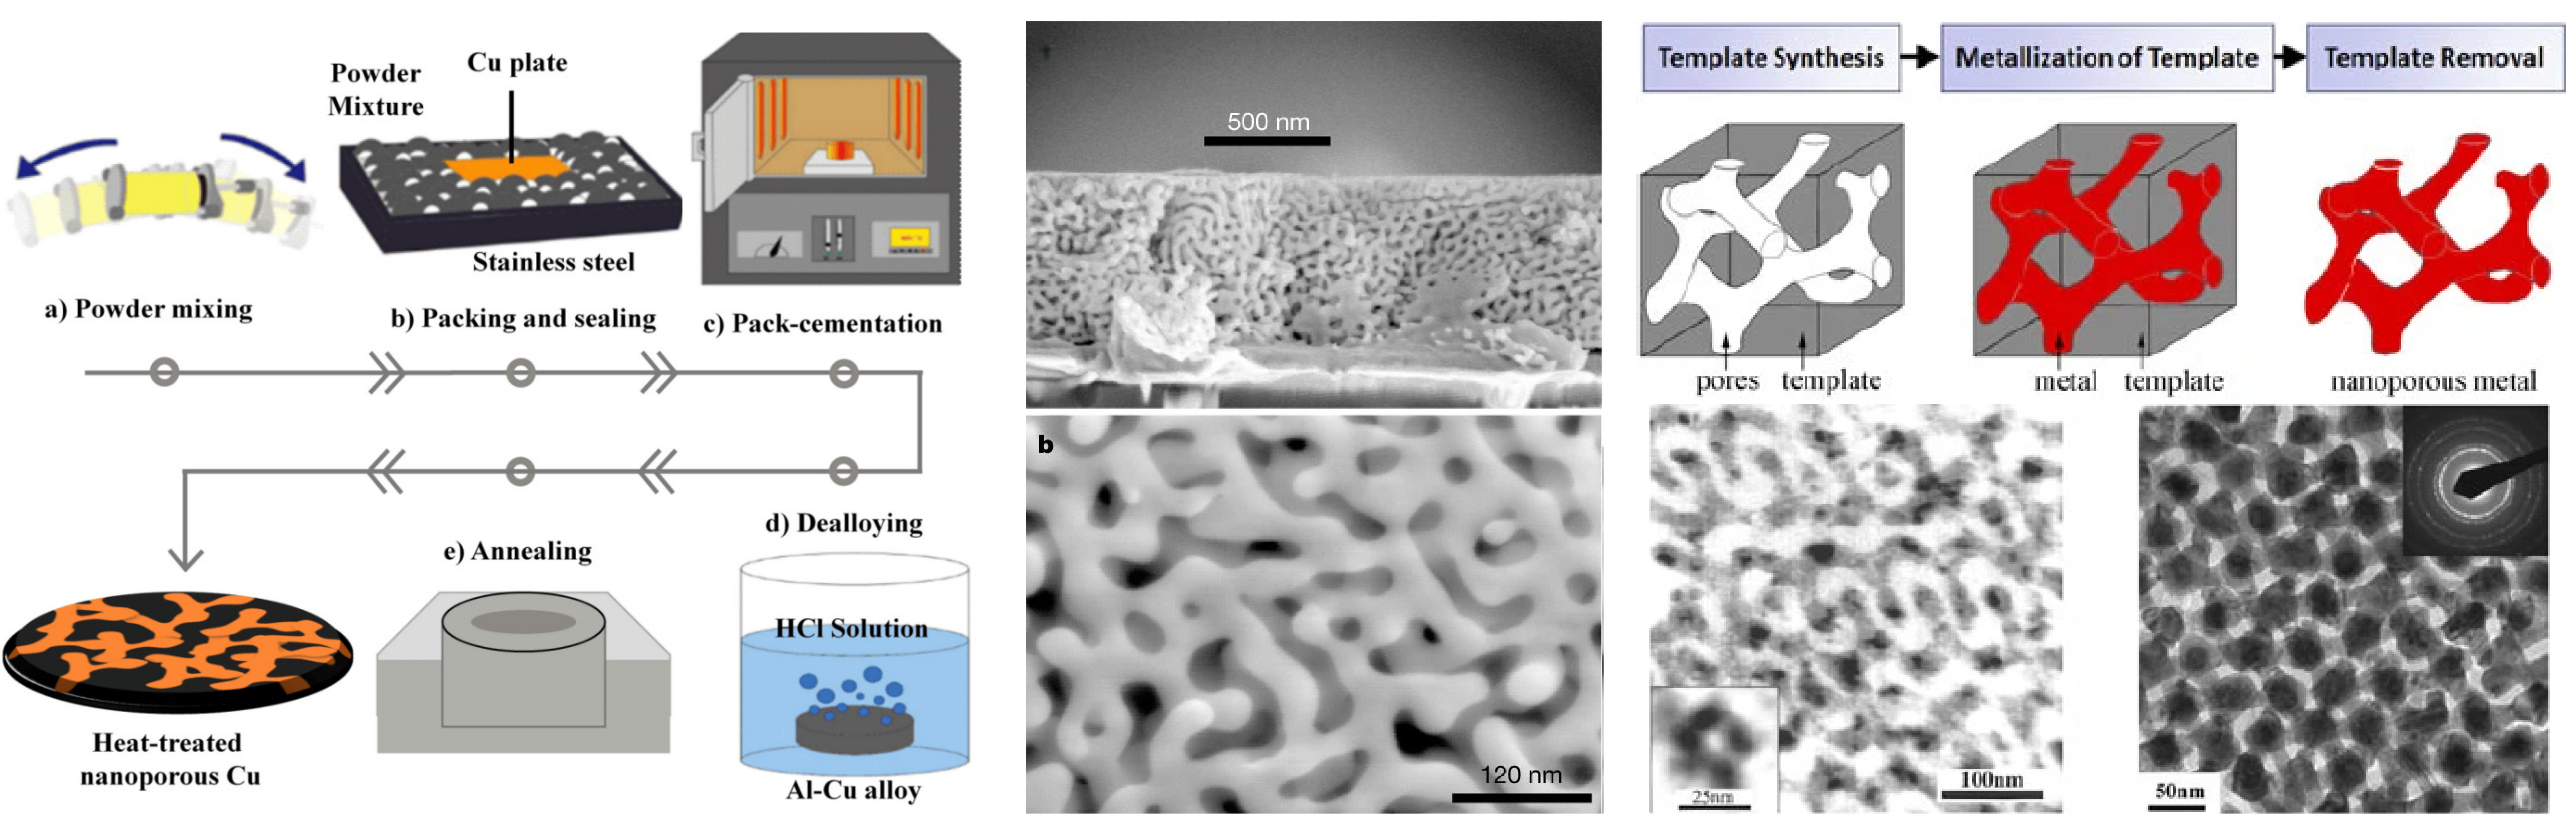
\includegraphics[width=1\linewidth]{photos/how2nanofoam.png}
    \caption{ a) Schematic process of dealloying of an Al-Cu Alloy \cite{Liu2020CuNanofoam}. b) Cross-section of dealloyed Au32$\%$Ag68$\%$ thin film. c) Schematic process and results of template-based fabrication of nanoporous metals \cite{Rebbecchi2018TemplateNanoporousMetals}.}
    \label{fig:how2nanofoam}
\end{figure}
\begin{figure} [H]
    \centering
    \includegraphics[width=0.9\linewidth]{photos/SCBD.png}
    \caption{a) Schematic representation of the two-source SCBD apparatus used in \cite{Profumo2021Neuromorphic}. b) Schematic representation of a nanocomposite Au/ZrOx film-based device.}
    \label{fig:SCBD}
\end{figure}

Metallic nanofoams can be synthesised using various techniques, generally classified into top-down approaches (dealloying \cite{Erlebacher2001Dealloying}, template-assisted methods \cite{Rebbecchi2018TemplateNanoporousMetals, Lee2006Electrodeposition}, some of them shown in Figure \ref{fig:how2nanofoam}) and bottom-up approaches (combustion synthesis \cite{Tappan2005Combustion}, supersonic cluster beam deposition – SCBD \cite{Profumo2021Neuromorphic, Benetti2018Nanometrology}). Dealloying selectively removes components of a binder to achieve controlled porosity; template-assisted methods use a sacrificial skeleton to shape the structure; electrodeposition in porous matrices allows precise control of pores and bonds; SCBD, whose experimental apparatus is shown in Figure \ref{fig:SCBD}, directly assembles metal clusters into three-dimensional nanostructures; combustion synthesis exploits exothermic reactions to generate a porous network. Each technique offers specific advantages in terms of morphological control, scalability and structure quality.






\section{My work}
Modelling thermal transport in metallic systems is a central challenge in modern materials science for a wide range of applications. Local disorder and size effects strongly influence heat transport, making traditional continuum or bulk-based models often insufficient to capture the underlying physics.\bigskip

This thesis studies how the phononic contribution to thermal conductivity varies across a multitude of Au-configurations: from the perfect bulk configuration to highly nanostructured assemblies, including nanopillars and nanofoams. In particular, the presented work explores the impact of porosity-driven defects on the overall thermal conductivity, including randomly distributed vacancies, spherical holes, and central voids, and sees how these initial systems can be used to parametrise assembled nanoparticle structures. 

To quantify the phononic contribution to thermal transport, we employ Equilibrium Molecular Dynamics (EMD) simulations, combining them with the Green–Kubo (GK) method to compute thermal conductivity. The full methodology is detailed in Chapter \ref{chap:md}. GK's method is the one that can also be extended to nanostructured systems, since it does not require a parametrisation of phonons into wave modes, which is not feasible when periodicity is disrupted.\bigskip 

To successfully compute the thermal conductivity, we develop a complete atomistic workflow that includes all stages of the simulation and analysis, extensively described in Chapter \ref{chap:mywork}. This includes the construction and manipulation of atomic configurations using ASE, the execution of EMD simulations in LAMMPS, and the final post-processing analysis. Python was employed for post-processing routines, utilising libraries like NumPy and Pandas to extract heat flux from the simulation output files, compute the autocorrelation functions, and integrate them according to the GK formalism to obtain the thermal conductivity. Additional structural analyses, including coordination numbers and porosity profiles, were also performed to correlate atomic-scale features with thermal transport.\bigskip

Overall, this thesis demonstrates that meaningful estimates of thermal conductivity can be obtained with the GK method even for complex, nanostructured systems that deviate from ideal crystalline assumptions. As summarised in Chapter 4, the results highlight the central role of porosity and local coordination in influencing thermal transport and illustrate how similar atomic fractions arranged in different topologies can lead to different thermal behaviour. 
    \chapter{Computer Simulations} \label{chap:md}
In recent decades, computer experiments have acquired a central role in many areas of physics, chemistry, and materials engineering. Their strength lies in the ability to bridge the gap between theory and experiment by transforming theoretical predictions into quantitative results that can be directly compared with experimental data, allowing each to inform and refine the other. 

Simulations act as a 'numerical laboratory' in which theoretical predictions can be tested, and when exact theories fail, they can reveal which approximations hold, helping physicists develop new models. At the same time, simulations can replicate laboratory experiments, allowing for direct comparison of results and a better understanding of behaviours that may be difficult to observe experimentally, such as the individual motions of atoms or molecules. Finally, simulations allow us to study systems under extreme conditions, which are both very hard to model theoretically and difficult to access experimentally.\\

\begin{figure}[H]
    \centering
    \includegraphics[width=0.8\textwidth]{photos/SIM-TEO-EXP_v2.png}
    \caption{The role of computer simulations in material discovery.}
    \label{fig:md_algorithm}
\end{figure}

There are many types of simulation, but among them, two stand out as the most effective for modelling systems of many interacting particles, both grounded in fundamental principles of statistical mechanics: Molecular Dynamics (MD) and Monte Carlo (MC). 
Their widespread adoption stems from their ability to handle systems with a large number of degrees of freedom, capturing both microscopic interactions and emergent macroscopic properties. While both aim to explore the behaviour of many-particle systems, they differ fundamentally in their approach: Molecular Dynamics follows deterministic trajectories obtained by integrating Newton’s equations of motion, whereas Monte Carlo relies on stochastic sampling to generate representative configurations according to statistical ensembles.\\

In the context of this work, the focus will be primarily on Molecular Dynamics, due to its ability to reproduce the time evolution of atomic and molecular systems with high fidelity. This makes it particularly well-suited for investigating transport properties, like thermal conductivity. The method provides direct access to trajectories in both real and phase space, from which thermodynamic quantities can be computed and microscopic mechanisms analysed in detail. To perform the simulations presented in this study, the open-source molecular dynamics package LAMMPS was employed, offering a flexible framework for implementing a variety of interatomic potentials, boundary conditions, and statistical ensembles.


\section{Molecular Dynamics}
Molecular Dynamics (MD) is a powerful simulation technique which allows the study of complex many-body systems at the atomic and molecular scale. This approach is based on the numerical integration of Newton’s equations of motion for a set of interacting particles. Each particle experiences forces derived from an interatomic potential, which can take different forms, ranging from simple two-body interactions to more sophisticated many-body descriptions, and can also express classical approximations of the underlying quantum mechanical interactions. \\

Molecular Dynamics was developed during the late 1950s and early 1960s, with the initial computer simulations of particle interactions. A significant achievement was the research conducted by Alder and Wainwright in 1957 at Lawrence Livermore National Laboratory, who utilised hard-sphere models to investigate phase transitions \cite{Alder1957}. This was followed by Rahman's groundbreaking simulation of liquid argon in 1964, which showcased the capabilities of molecular dynamics for realistic modelling of condensed matter systems \cite{Rahman1964}. During the 1970s and 1980s, the introduction of more precise interatomic potentials and improvements in numerical algorithms enhanced the usefulness of MD for studying biomolecules, polymers, and complex fluids. The recent increase in computational capability has allowed molecular dynamics to evolve into an even more reliable technique, enabling the simulation of highly complex systems with millions of atoms over timescales, ranging from nanoseconds to microseconds.\\

Therefore, by tracking the instantaneous positions of the particles, MD becomes a powerful tool for investigating the microscopic behaviour of matter and, through the computation of ensemble averages, for establishing its connection with macroscopic thermodynamic properties such as temperature, pressure, diffusion coefficients, and thermal conductivity. To fully understand its capabilities, it is important to investigate more thoroughly how it functions and what key characteristics a reliable MD algorithm should include.


\section{MD Algorithms}
The best way to introduce Molecular Dynamics is to consider a simple program, which shows what are the key points of this kind of simulation. The program is built as follows:

\begin{enumerate}
    \item We input the parameters specifying the simulation conditions, like the number of particles, time step, temperature, etc. They play an important role in the simulation and strongly influence its accuracy and efficiency.
    \item We set the initial position and velocity of each particle; this step is called initialisation.
    \item We compute the forces acting on all particles.
    \item We integrate Newton's equation of motion. These and the previous steps are the core of the algorithm, and they are repeated until we have evolved our system for the desired length of time.
    \item We compute the averages of measured quantities and stop the simulation.
\end{enumerate}

\begin{figure}[H] % [H] forza la posizione qui, serve il package float
    \centering
    \includegraphics[width=0.7\textwidth]{photos/md_algorithm.png}
    \caption{Schematic representation of a typical MD algorithm \cite{frenkel_smit}.}
    \label{fig:md_algorithm}
\end{figure}

 This short pseudo-algorithm, shown in Figure \ref{fig:md_algorithm}, is able to carry out a Molecular Dynamics simulation for a simple atomic system, but it contains all the crucial points that every MD script should have, even the more sophisticated ones.  

\subsection{Initialization}
The initialisation phase represents the starting point of any Molecular Dynamics simulation. In this step, initial positions and velocities must be assigned to all particles in the system, in a way that reflects the structure we intend to simulate (Figure \ref{fig:pos_init}). Positions in particular must be chosen avoiding unrealistic overlaps between atomic or molecular cores. Proper initialisation ensures that the system begins its evolution from a physically meaningful configuration, preventing instabilities and unphysical results during the dynamics. 

\begin{figure}[H]
    \centering
    \includegraphics[width=0.7\textwidth]{photos/pos_init.png}
    \caption{Typical MD initial structures: crystal lattice, amorphous arrangement, and biomolecule (biomolecule of the month, November 2025 \cite{pdb, Berman2000PDB})}
    \label{fig:pos_init}
\end{figure}

Another crucial aspect to consider during initialisation is the treatment of the system boundaries. In Molecular Dynamics simulations, it is common to employ periodic boundary conditions (PBC) to mimic an effectively infinite system and avoid surface effects. As shown in Figure \ref{fig:pbc}, with PBC, particles that move out of one side of the simulation box re-enter from the opposite side, ensuring that the density and structure of the system remain consistent. 

\begin{figure}[H]
    \centering
    \includegraphics[width=1\linewidth]{photos/pbc.png}
    \caption{Periodic Boundary Conditions (PBC), example in two dimensions. The darker region is the simulation box, while the surrounding squares are the periodically repeated images. The arrows identify an atom crossing through a boundary and re-entering the box on the opposite side.}
    \label{fig:pbc}
\end{figure}

Once the particle positions are defined, it's time to assign the initial velocities. This is typically done according to the Maxwell–Boltzmann distribution at the desired simulation temperature. This ensures that the system’s kinetic energy is consistent with the target thermodynamic conditions predicted by statistical mechanics.

As another option, one can initialise all particle velocities to zero and slowly adjust the system to the desired temperature using a thermostat. This method, commonly referred to as thermalisation or equilibration, enables the system to achieve a realistic distribution of kinetic energy without causing significant initial forces that may destabilise the simulation. Gradually raising the temperature promotes a gentle transition from the starting configuration and minimises the potential for numerical instabilities, particularly in dense or highly interactive systems.


\subsection{The Force Calculation}
What comes next is the most time-consuming part of the typical Molecular Dynamics algorithm: computing all the forces acting upon each particle. The forces are derived from an interatomic potential, which defines how particles interact with each other. Depending on the system under study, these potentials can range from simple pairwise interactions, such as the Lennard–Jones potential \cite{jones1924}, to more sophisticated many-body formulations like the Embedded Atom Method (EAM) \cite{daw1984eam} or reactive force fields (ReaxFF) \cite{vanduin2001}. The accuracy of a Molecular Dynamics simulation strongly depends on the choice of the potential. A well-chosen potential captures the essential physics of the material, while a poor choice can lead to unrealistic results.\\

In this study, the interactions among gold atoms are simulated using the Embedded Atom Method (EAM), a many-body potential that has been specifically designed for metallic systems \cite{foiles1986eamfcc}. Unlike basic pairwise models, which rely solely on the separation between two atoms, EAM considers that an atom's energy in a metal is influenced not only by its pairwise interactions but also by the local electron density generated by its neighbours. This characteristic makes EAM particularly effective for accurately capturing the cohesive properties, elastic behaviour of conductive metals like gold. 
The total potential energy of the system is expressed as

\begin{equation}
PE_{\text{tot}} = \sum_{i} F\!\left(\rho_i\right) + \frac{1}{2}\sum_{i \neq j} \phi(r_{ij})
\end{equation}

 where:
\begin{itemize}
    \item $F(\rho_i)$ is the \textit{embedding energy}, i.e. the energy cost to embed atom $i$ into the local electron density $\rho_i$,
    \item $\rho_i = \sum_{j \neq i} f(r_{ij})$ is the \textit{host electron density} at the position of atom $i$, obtained as a superposition of atomic electron density contributions $f(r_{ij})$ from neighbouring atoms,
    \item $\phi(r_{ij})$ is a \textit{pairwise potential} describing electrostatic and repulsive core interactions,
    \item $r_{ij}$ is the distance between atoms $i$ and $j$.
\end{itemize}

The \textit{force} on atom $i$ is then derived from the negative gradient of the total energy:

\begin{equation}
\mathbf{F}_i = - \nabla_{\mathbf{r}_i} PE_{\text{tot}}= - \sum_{j \neq i} \left[ F'(\rho_i)\, f'(r_{ij}) + F'(\rho_j)\, f'(r_{ij}) + \phi'(r_{ij}) \right] \hat{\mathbf{r}}_{ij}
\end{equation}

where $\hat{\mathbf{r}}_{ij} = \frac{\mathbf{r}_i - \mathbf{r}_j}{r_{ij}}$ is the unit vector along the $i-j$ direction, and primes denote derivatives with respect to the argument.\\

This formulation highlights the many-body nature of the EAM: the force on each atom depends not only on its pairwise interactions but also on the electron density contributions from the entire neighbourhood.\\

Given that the determination of forces needs to be performed at each integration step, the efficiency of this process greatly influences the overall practicality of a molecular dynamics simulation. Thus, let’s examine the computational expense related to force evaluation. 

If we consider a model system with pairwise additive interactions, we have to consider the contribution to the force on particle $i$ due to all its neighbours, keeping in mind PBCs. If we consider only the interaction between a particle and the nearest image of another particle, this implies that, for a system of $N$ particles, we must evaluate $N \times (N-1)/2$ pair distances.
This implies that, if we use no tricks, the time needed for the evaluation of the forces scales as $N^2$. And since in EAM, in addition to the pairwise interactions, it is necessary to calculate and sum the electron density induced by all the neighbours of each atom, the time scaling is still $N^2$ but the prefactor is larger than for a simple two-body potential like Lennard-Jones, because the per-particle calculations are more complex. \\

To reduce the computational cost, it is common to introduce a cut-off radius, $r_\text{cut}$, beyond which interactions are neglected. This reduces the number of pair distances that need to be evaluated for each atom, effectively lowering the scaling from $O(N^2)$ to approximately $O(N)$ for short-range potentials \cite{rapaport2004}.
Furthermore, the use of neighbour lists allows us to keep track of only those particles within the cut-off distance for each atom, avoiding unnecessary distance calculations at every time step. 

These techniques are essential for making large-scale molecular dynamics simulations feasible, especially when dealing with many-body potentials like EAM; however, it is important to note that introducing a cut-off and using approximations introduces small errors in the force evaluation. Therefore, there is always a trade-off between computational efficiency and accuracy, and the choice of cut-off radius or other approximations must balance performance with the level of precision required.\\


\subsection{Integrating the Equation of Motion}
Now that all forces between the particles are computed, it's time to integrate Newton's equation of motion to update particle positions and velocities. The integration of the equations of motion is done at each time step to move the system from its current configuration to the next. 

Firstly, the choice of the time step $\Delta t$ is crucial: it must be small enough to accurately show the fastest motions in the system, while large enough to allow the simulation to reach meaningful timescales in a reasonable computational time.

Secondly, to achieve an effective simulation, an appropriate integration algorithm needs to be selected. Before discussing what are the most utilised methods, it's better to understand what makes a good integration algorithm. Contrary to what someone might think, speed is less critical (since force calculations dominate computational cost), while accuracy at larger time steps is highly important: the longer the time step an algorithm allows without losing stability, the fewer force evaluations are needed. Such algorithms achieve this by storing higher-order derivatives of particle coordinates. Ideally, the perfect algorithm should be able to predict particle trajectories accurately over both short and long times. However, due to Lyapunov instability, small differences between the exact trajectory and the simulated one grow exponentially over time, making precise long-term trajectory prediction impossible. This, however, does not seriously compromise the usefulness of MD simulations, as statistical properties remain meaningful. 

Energy conservation is another key feature. High-order algorithms often conserve energy very well over short times but can exhibit energy drift in the long-term, whereas simpler algorithms may be less accurate short-term but maintain much better long-term energy stability. Thus, a good integration algorithm balances the ability to use reasonably large time steps, stable energy behaviour, and numerical simplicity. \\

One of the most widely used integration algorithms that combines computational efficiency, numerical stability, and energy conservation is the Verlet algorithm \cite{Verlet1967}. It can be easily obtained from the Taylor expansion of the coordinate of a particle around time $t$: 
\begin{equation}
\begin{split}
    r(t+\Delta t) = r(t) + v(t) \Delta t + \frac{1}{2}a(t)\Delta t^2 + \frac{\Delta t^3}{3!} \dot a(t)+ \mathcal{O}(\Delta t^4) \\
    r(t-\Delta t) = r(t) - v(t) \Delta t + \frac{1}{2}a(t)\Delta t^2 - \frac{\Delta t^3}{3!} \dot a(t)+ \mathcal{O}(\Delta t^4)
    \label{eq:r_expansion}
\end{split}
\end{equation}

 Summing the two previous equations:
\begin{equation}
    r(t+\Delta t) = 2r(t) + r(t-\Delta t) + a(t)\Delta t^2 + \mathcal{O}(\Delta t^4)
    \label{eq:verlet_r_update}
\end{equation}

 The estimation of the new position is calculated with an error of the order of $\Delta t^4$ and contains the information of the previous two steps, thus making this algorithm highly correlated. Also, it's important to note that the algorithm does not use the velocity to compute the new position; however, it can be derived from the knowledge of the trajectory:
\begin{equation*}
    r(t+\Delta t) - r(t-\Delta t) = 2v(t)\Delta t  + \mathcal{O}(\Delta t^4)
\end{equation*}
 or
\begin{equation}
    v(t) = \frac{r(t+\Delta t) - r(t-\Delta t)}{2\Delta t}  + \mathcal{O}(\Delta t^2)
    \label{eq:verlet_v_calc}
\end{equation}

Now that we have computed the new positions, we can discard the positions at $t-\Delta t$. The current positions become the old ones, and the new positions become the current positions, and we can move on to the next step. \\

There exist several alternatives to the basic Verlet integration algorithm, including the Leapfrog algorithm and the Velocity-Verlet algorithm \cite{frenkel_smit}. In this work, we focus on the latter, as the Velocity-Verlet scheme is the default integration algorithm used in LAMMPS \cite{lammps_velocity_verlet}. Unlike the basic Verlet, it explicitly incorporates velocity updates at each step. This method preserves the advantages of the Verlet scheme (simplicity, time reversibility, and good energy conservation) while providing a direct evaluation of velocities, which is often required in molecular dynamics (computing kinetic energy, temperature, or applying thermostats). The Velocity-Verlet algorithm can be obtained as follows.\\


We start from the position update in equation \eqref{eq:verlet_r_update} and the velocity calculation in equation \eqref{eq:verlet_v_calc} provided by the classical Verlet algorithm. But we want an update that advances $v$ consistently from $t$ to $t+\Delta t$, so expand $v$ and $a$ in time:
\begin{equation*}
\begin{split}
v(t+\Delta t) &= v(t) + a(t)\,\Delta t + \tfrac{1}{2}\dot a(t)\,\Delta t^2 + \mathcal{O}(\Delta t^3) \\
a(t+\Delta t) &= a(t) + \dot a(t)\,\Delta t + \mathcal{O}(\Delta t^2)
\end{split}
\end{equation*}
Eliminate $\dot a(t)$ between the two previous equations:
\[
\tfrac{1}{2}\dot a(t)\,\Delta t^2 \;=\; \tfrac{1}{2}\big[a(t+\Delta t)-a(t)\big]\Delta t + \mathcal{O}(\Delta t^3).
\]
Substituting in velocity expansion yields the velocity update
\begin{equation*}
v(t+\Delta t) \;=\; v(t) + \tfrac{1}{2}\big[a(t)+a(t+\Delta t)\big]\Delta t + \mathcal{O}(\Delta t^3).
\label{eq:vv-velocity}
\end{equation*}

Combining the $\mathcal{O}(\Delta t^2)$ position advance from \eqref{eq:r_expansion} (truncated at second order) with \eqref{eq:vv-velocity} gives the Velocity--Verlet algorithm:
\begin{align}
\text{(i)} \quad & r(t+\Delta t) = r(t) + v(t)\,\Delta t + \tfrac{1}{2}a(t)\,\Delta t^2 \label{eq:vv-pos}\\
\text{(ii)}\quad & \text{Compute } a(t+\Delta t) = \frac{F\big(r(t+\Delta t)\big)}{m} \nonumber\\
\text{(iii)}\quad & v(t+\Delta t) = v(t) + \tfrac{1}{2}\big[a(t)+a(t+\Delta t)\big]\Delta t \label{eq:vv-vel}
\end{align}

An equivalent ``half-step'' form underlines the staggered velocity update:
\begin{align*}
v\!\!\left(t+\tfrac{\Delta t}{2}\right) &= v(t) + \tfrac{1}{2}a(t)\,\Delta t \\
r(t+\Delta t) &= r(t) + v\!\left(t+\tfrac{\Delta t}{2}\right)\Delta t \\
v(t+\Delta t) &= v\!\left(t+\tfrac{\Delta t}{2}\right) + \tfrac{1}{2}a(t+\Delta t)\,\Delta t
\end{align*}

The positions are updated using the current velocities and forces, while the velocities are updated in two half-steps: first using the forces at time $t$, and then corrected with the forces at $t+\Delta t$. This half-step Velocity-Verlet formulation is the one implemented in LAMMPS, ensuring that positions and velocities remain synchronised in time, which makes the algorithm efficient and convenient for practical simulations.

\section{LAMMPS}
The Large-scale Atomic/Molecular Massively Parallel Simulator (LAMMPS) is an open-source software package used widely for molecular dynamics (MD) simulations. 
It was originally developed in the mid-1990s under a 5-way cooperative research between Sandia National Laboratories and Lawrence Livermore National Laboratory and three companies (Cray, DuPont, and Bristol-Myers Squibb). The goal was to create a parallel molecular dynamics code capable of running on large supercomputers for modelling materials and biomolecules. Initially written in Fortran, LAMMPS was later rewritten in C++ to provide greater flexibility and ease of adding new functionality \cite{lammps_history}.
Since its creation, LAMMPS has evolved into one of the most popular and flexible MD codes in the scientific community, supported by a large user base and continuous contributions from both academia and industry. Developers can contribute directly to the LAMMPS source code, customising it or adding new features and algorithms through a modular design. 

\subsection{Parallelization and Performance}
As said in the introduction, LAMMPS was designed with parallel scalability in mind, allowing efficient use of computational resources, ranging from a single processor on a laptop to massively parallel supercomputers with thousands of cores or even GPU accelerators. This scalability is possible thanks to the fact that the code uses a technique called domain decomposition or partitioning, where the simulation box is separated into non-overlapping subdomains which fill the box and each assigned to a processor.\\

Based on the spatial distribution of the particles to be simulated, the simulation box can be divided in different ways, as shown in Figure \ref{fig:domain_decomp}. 

When the particle density is roughly uniform, the subdomains comprise a regular grid and all subdomains are identical in size and shape, containing roughly the same number of atoms. Both orthogonal and triclinic boxes can deform continuously during a simulation, for example, when simulating the compression of a solid or the shearing of a liquid, in which case the processor subdomains also deform.

For systems with non-uniform density, with the default partitioning, the number of particles per processor can be imbalanced. This reduces parallel efficiency, as the overall simulation rate is limited by the slowest processor, i.e. the one with the largest computational load. For such models, LAMMPS supports multiple strategies to reduce the load imbalance.

\begin{figure}[H]
    \centering
    \includegraphics[width=0.9\textwidth]{photos/domain_decomp.png}
    \caption{Three kinds of spatial decomposition (partitioning) of the simulation box for MPI parallelism \cite{lammps_balance}.}
    \label{fig:domain_decomp}
\end{figure}

Next to spatial decomposition, LAMMPS uses other advanced algorithms to handle particle interactions in large systems. Neighbour lists that track the neighbours of each particle within a cutoff radius, allowing forces to be calculated only between particles that are actually close together. For long-range interactions, like Coulombic interactions, LAMMPS implements efficient methods based on parallel FFTs \cite{press2007numerical} or Ewald \cite{Ewald1921} and PPPM techniques \cite{hockney_eastwood_1988}, allowing systems with thousands or millions of particles to be handled without sacrificing accuracy. 


\subsection{Input Style}
One of the key features of LAMMPS is the ease of interaction with the executable. This is achieved primarily through input scripts, text files containing a sequence of commands.
These commands, extensively described in the LAMMPS wiki, define the system (units, atom styles, force fields), the simulation configuration (neighbour lists, integration algorithms, corrections), and the desired outputs (thermodynamic quantities, dumps, calculations).
The input style is command-driven and modular: each line corresponds to a specific task, and commands can be combined or extended via additional packages. This approach makes LAMMPS highly flexible and intuitive for scripting complex workflows. 

Once executed, the input file is parsed line by line by the LAMMPS engine. Within the executable, the corresponding modules are activated and combined with the chosen parallelisation strategy. %For example, running the same script on a single core or across hundreds of processors does not require modifying the input file; LAMMPS automatically manages the distribution of data and calculations \GB{while leaving to the user the ability to define how the simulation box is to be divided among the processors}. Similarly, when GPU acceleration is enabled, computationally intensive tasks such as pairwise force calculations are offloaded to the GPU, maintaining the same input syntax \GB{though in the case of GPU acceleration is advisable to specify appropriately defined interaction potentials optimized to run on GPUs}. 
This separation between the input description and the underlying architecture is one of the main reasons LAMMPS is widely adopted: it allows researchers to focus on the physics problem without having to worry about low-level implementation details.\\

Beyond defining the system and computational resources, the input scripts allow precise control over the simulation dynamics. Users can select among a wide range of interatomic potentials, from simple pairwise potentials such as Lennard-Jones to more complex many-body models like Embedded Atom Method (EAM) or Tersoff \cite{Tersoff1986}, enabling simulations of metals, semiconductors, and hybrid systems. Additionally, integration schemes such as Velocity-Verlet or Leapfrog can be chosen, and thermostats or barostats (e.g., Nosé-Hoover \cite{Hoover1985} or Langevin \cite{Berne1970, Langevin1908}) applied to maintain target temperatures or pressures, corresponding to NVE, NVT, or NPT ensembles. \\

The input file also governs the generation of output data and on-the-fly calculations. Thermodynamic quantities (temperature, energy, pressure) can be printed at specified intervals, while trajectories of particle positions, velocities, and forces can be dumped for post-processing. Users can further instruct LAMMPS to compute per-atom properties, stress tensors, radial distribution functions, or heat fluxes during the simulation. By integrating system definition, simulation control, and output specification within a single script, LAMMPS ensures flexibility, reproducibility, and ease of use for complex simulation workflows.


\subsection{Extensions and Community}
LAMMPS features a modular architecture that enables users to enhance its core functions through optional packages. These packages offer specialised features, including advanced interatomic potentials like MEAM \cite{baskes1992} and many-body potentials, as well as high-performance computing improvements such as GPU or OpenMP acceleration. 
The open-source nature of LAMMPS has created an active community of developers and users. Contributions from both academic and industrial sectors continuously extend the code with new algorithms, interatomic potentials, and analysis tools. For example, the integration of machine-learning frameworks such as FLARE \cite{Vandermause2020} allows on-the-fly training of interatomic potentials, while platforms like OpenKIM \cite{openkim_lammps_tutorial} provide standardised tests and pre-defined potentials, facilitating reproducible and reliable simulations.\\

Importantly, no contributed feature is incorporated into LAMMPS without proper documentation \cite{lammps_doc}. The manual includes a dedicated Programmer's Guide, which explains the structure of the source code and provides guidance on extending or modifying its functionality. 
Additionally, users can benefit from forums \cite{LAMMPS_Forum_40}, mailing lists, and a comprehensive wiki, where shared examples, tutorials, and scripts are available, promoting collaboration, reproducibility, and knowledge exchange within the community. 
Together, these characteristics make LAMMPS highly accessible and user-friendly, even for complex simulation tasks. 


\section{LAMMPS Thermodynamic Calculations}

Once a molecular dynamics simulation is initialised and the system evolves in time, LAMMPS provides access to a variety of microscopic data, such as atomic positions, velocities, and forces. Macroscopic thermodynamic quantities can then be computed from these microscopic variables, either instantaneously or as time averages, following the principles of statistical mechanics. These quantities are only calculated when explicitly requested, for example, through specific commands, fixes, or computes that require them. 


\subsection{Temperature}
In LAMMPS, the temperature is computed from the atomic velocities according to the equipartition theorem of classical statistical mechanics. 
The theorem states that each quadratic degree of freedom contributes, on average, an energy of $\tfrac{1}{2}k_BT$ to the system. 
For $N$ atoms in three dimensions, there are $3N$ translational degrees of freedom, leading to an average kinetic energy
\begin{equation*}
    \langle K \rangle = \frac{3}{2} N k_B T.
\end{equation*}

From this relation, the instantaneous temperature is defined through the kinetic energy of the system as
\begin{equation}
    T = \frac{2}{3 N_{\mathrm{dof}} k_B} \sum_{i=1}^N \frac{1}{2} m_i v_i^2 ,
\end{equation}
where $N_{\mathrm{dof}}$ is the number of active degrees of freedom, which may be smaller than $3N$ if constraints or fixed atoms are present. 
LAMMPS automatically subtracts the degrees of freedom associated with constraints and rigid-body fixes when evaluating the temperature. 
The instantaneous value of $T$ can be printed with \texttt{thermo\_style} by including the keyword \texttt{temp}, or accessed via a compute of type \texttt{compute temp}, which calculates the kinetic temperature of a specified group of atoms.

It is worth stressing that this classical definition holds under the assumption of full equipartition. At sufficiently low temperatures, quantum effects may suppress certain vibrational contributions, leading to deviations from the classical prediction; such effects are not captured within the standard classical MD framework implemented in LAMMPS.

\subsection{Pressure}
The pressure in a molecular system can be derived from the virial theorem, which relates the average scalar product between positions and forces to the kinetic energy as
\begin{equation*}
\left\langle \sum_{i=1}^N \mathbf{r}_i \cdot \mathbf{F}_i \right\rangle = -2 \langle K \rangle
\end{equation*}
where $K$ is the total kinetic energy. For a cubic simulation box of volume $V$, one can combine this relation with the mechanical definition of pressure as momentum transfer at the boundaries to obtain
\begin{equation*}
P = \frac{1}{3V} \left( 2K + \sum_{i=1}^N \mathbf{r}_i \cdot \mathbf{F}_i \right).
\end{equation*}
Expressing the kinetic energy via the equipartition theorem, $K = \tfrac{3}{2}Nk_BT$, leads to the microscopic expression for the instantaneous pressure:
\begin{equation}
P = \frac{Nk_B T}{V} + \frac{1}{3V} \sum_{i=1}^N \mathbf{r}_i \cdot \mathbf{F}_i 
\end{equation}
The first term corresponds to the ideal gas contribution, while the second arises from interatomic interactions and vanishes for a non-interacting system, recovering the ideal gas law.  

In LAMMPS, this virial expression is implemented internally and can be accessed through the command \texttt{compute pressure}
 or the keyword \texttt{press} in the \texttt{thermo\_style} command, or more generally via the global thermodynamic quantities computed at each timestep. Pressure is thus obtained consistently with the force field in use, automatically accounting for pairwise, bonded, and long-range interactions, as well as any imposed constraints. 


\subsection{Energy}
The total energy of the system is given by the sum of kinetic and potential contributions:
\begin{equation}
E = KE + PE
\end{equation}
with
\begin{equation}
KE = \sum_{i=1}^N \frac{1}{2} m_i v_i^2
\quad \quad
PE = \sum_{i<j} U(r_{ij})
\end{equation}

Usually, the kinetic energy of each particle is computed as $\tfrac{1}{2} m v^2$, where $m$ and $v$ are the mass and velocity of the particle, respectively. But in reality, there are two different ways to compute the kinetic energy, both coherently integrated within LAMMPS. The one evaluated from the expression above is the so-called translational kinetic energy, tied to the velocity of all the particles in the system. In thermodynamic output, it is often calculated from the instantaneous temperature of the system using the equipartition theorem, which simply assigns $\tfrac{1}{2}k_BT$ of energy for each quadratic degree of freedom. For the default definition of temperature, these two approaches coincide. However, more precise temperature calculations can subtract non-thermal components of motion (e.g., center-of-mass drift, rotation of a rigid body) or include different sets of degrees of freedom, leading to slightly different reported values of kinetic energy from the two methods.\\

The potential energy, on the other hand, is obtained from the interaction model specified for the system. Depending on the force field and the chosen interactions, the total $PE$ may include just the pairwise contributions $U(r_{ij})$, or include also more complicated terms as bond stretching, angle bending, torsional (dihedral), improper terms, as well as long-range interactions in reciprocal space (Ewald or PPPM) and additional energy terms introduced by hand. 
Obviously, given the complexity of these latter potentials, it is easy to imagine that the calculation of the PE could have an influence on the total computational cost of the simulation.\\

In molecular dynamics, $E$ provides information on the internal state of the system and is strictly conserved only in microcanonical ($NVE$) simulations with an ideal integrator. In practice, due to numerical errors, the total energy fluctuates around a mean value; monitoring its stability is a standard way to assess the quality of the integration scheme. In canonical ($NVT$) or isothermal–isobaric ($NPT$) simulations, $E$ is no longer conserved, but still provides useful insights: for instance, comparing average kinetic and potential energy contributions reveals how energy is partitioned between particle motion and interactions, and they reflect how the system couples to the thermostat or barostat.

\subsection{Stress tensor}
The stress tensor is crucial to understanding the link between atomistic forces and macroscopic mechanical quantities such as pressure, surface tension, and stress under deformation. In molecular simulations, it is usually defined through a virial expression that combines the kinetic contribution of particle momenta with the configurational part due to interatomic forces and can be seen as the tensor generalization of the same expression of pressure. The trace of this tensor is related to the thermodynamic pressure (via the virial theorem), while its off-diagonal elements quantify shear stresses and are central in the calculation of transport properties such as viscosity. 

In LAMMPS, the global stress tensor is obtained through the \texttt{compute pressure} command, which evaluates the virial expression by combining the kinetic term from a chosen temperature compute and the configurational term from interatomic forces. At the microscopic level, local virial contributions are calculated with two different computes, \texttt{compute stress/atom} and \texttt{compute centroid/stress/atom}, both of which follow the following formula, where $a$ and $b$ take on values $x,y,z$ to generate the components of the tensor:
\begin{equation}
    S_{ab} = -mv_av_b - W_{ab}
\end{equation}
where the first term is a kinetic energy contribution per atom and the second term is the virial, for which the compute style determines the exact computation details. Then, since these values correspond to a per-atom virial with units of energy, they must be divided by an appropriate volume to obtain a local stress field.

The first calculation method is \texttt{compute stress/atom}, where the tensor calculated for every atom is symmetric and consists of 6 components, represented as a 6-element vector in the sequence: $xx$, $yy$, $zz$, $xy$, $xz$, $yz$. In this scenario, the virial contribution is determined in the following manner:
\begin{equation}
\begin{split} 
W_{ab} & = \frac{1}{2} \sum_{n = 1}^{N_p} (r_{1_a} F_{1_b} + r_{2_a} F_{2_b}) + \frac{1}{2} \sum_{n = 1}^{N_b} (r_{1_a} F_{1_b} + r_{2_a} F_{2_b})  \\
& + \frac{1}{3} \sum_{n = 1}^{N_a} (r_{1_a} F_{1_b} + r_{2_a} F_{2_b} + r_{3_a} F_{3_b}) + \frac{1}{4} \sum_{n = 1}^{N_d} (r_{1_a} F_{1_b} + r_{2_a} F_{2_b} + r_{3_a} F_{3_b} + r_{4_a} F_{4_b}) \\
& + \frac{1}{4} \sum_{n = 1}^{N_i} (r_{1_a} F_{1_b} + r_{2_a} F_{2_b} + r_{3_a} F_{3_b} + r_{4_a} F_{4_b}) + \mathrm{Kspace}(r_{i_a},F_{i_b}) + \sum_{n = 1}^{N_f} r_{i_a} F_{i_b}
\end{split}
\end{equation}
The first term is a pairwise energy contribution where $n$ loops over the neighbours of each atom, $\textbf{r}_1$ and $\textbf{r}_2$ are the positions of the two atoms in the pairwise interaction, and $\textbf{F}_1$ and $\textbf{F}_1$ are the forces on the two atoms resulting from the pairwise interaction. The second term is a bond contribution of similar form for the $N_b$ bonds that the atom is part of. There are similar terms for the $N_a$ angle, $N_d$ dihedral, and $N_i$ improper interactions the atom is part of. There is also a term for the KSpace contribution from long-range Coulombic interactions, if defined. Finally, there is a term for the $N_f$ fixes (shake or rigid --Inserire links--) that apply internal constraint forces to the atom.

In case of compute \texttt{centroid/stress/atom}, the tensor computed for each atom is asymmetric with 9 components and is stored as a 9-element vector, and the virial contribution is:
\begin{equation}
    \begin{split} W_{ab} & = \sum_{n = 1}^{N_p} r_{I0_a} F_{I_b} + \sum_{n = 1}^{N_b} r_{I0_a} F_{I_b} + \sum_{n = 1}^{N_a} r_{I0_a}  F_{I_b} + \sum_{n = 1}^{N_d} r_{I0_a} F_{I_b} + \sum_{n = 1}^{N_i} r_{I0_a} F_{I_b} \\
& + \mathrm{Kspace}(r_{i_a},F_{i_b}) + \sum_{n = 1}^{N_f} r_{i_a} F_{i_b}\end{split}
\end{equation}
As for the other compute, the first, second, third, fourth and fifth terms are pairwise, bond, angle, dihedral and improper contributions, but instead of assigning the virial contribution equally to each atom, only the force $\textbf{F}_I$ acting on atom $I$ due to the interaction and the relative position $\textbf{r}_{I0}$ of the atom $I$ to the geometric center of the interacting atoms, i.e. centroid, is used. As the geometric center is different for each interaction, the $\textbf{r}_{I0}$ also differs. The sixth term, Kspace contribution, is computed identically to \texttt{compute stress/atom}. 

Because of the two distinct methods for calculating the stress tensor, there are some variations in the results: while the total system virial remains the same as when using \texttt{compute stress/atom}, the \texttt{compute centroid/stress/atom} method is recognized for yielding more reliable heat flux values for angle, dihedrals, improper, and constraint force contributions when evaluated using \texttt{compute heat/flux}.


\subsection{Heat Flux}
In simulations, the microscopic heat flux quantifies the rate at which energy is transported through the system. LAMMPS provides an easy way to compute it via the command \texttt{compute heat/flux}, which takes the per-atom values of kinetic energy, potential energy, and the stress tensor as input and returns a three-dimensional vector. For a system of $N$ particles with pairwise interactions occupying a volume $V$, the heat flux is:

\begin{equation}
    \mathbf{J} = \frac{1}{V} \left[ \sum_{i=1}^N e_i \mathbf{v}_i - \sum_{i=1}^N  \mathbf{S}_{i} \mathbf{v}_i \right]
\end{equation}
in the first term $e_i = \tfrac{1}{2}m_i v_i^2 + u_i$ is the per-atom energy, where $u_i$ is a suitable partition of the potential energy among atoms, which can be complex to deal with. In the case of many-body or bonding potentials (e.g., Embedded Atom Model, Tersoff,...), the decomposition of the potential energy $PE$ into per-atom contributions $u_i$ is not unique. For simple pairwise interactions, each atom can be assigned half the interaction energy with all its neighbours, $u_i = \tfrac{1}{2}\sum_{j\neq i} U(r_{ij})$.
However, for many-body potentials, the energy depends on the local environment of each atom and cannot be uniquely assigned to pairs. Several conventions exist for defining $u_i$, but they must be consistent with the forces, so that the energy partitioning exactly reproduces the total potential energy and forces used in the simulation. The second term involves the atomic stress tensor $\textbf{S}_i$. While the virial expression is straightforward for pairwise interactions, many-body potentials require additional terms, and the atomic stress must be computed using a force decomposition consistent with the potential.

Even though the microscopic definitions of per-atom energy $u_i$ and stress $\textbf{S}_i$ are not unique, the macroscopic behaviour of the system remains invariant. This means that, while different conventions may lead to different microscopic partitions, any physically meaningful, system-wide observable calculated from these quantities converges to the same result in the thermodynamic limit.


\subsection{Transport Properties}
Transport properties characterise how a system responds to gradients in momentum, energy, or particle concentration. They provide a direct link between the microscopic motion of individual particles and macroscopic observables such as diffusion coefficients, viscosity, or thermal conductivity. By analysing these properties, it is possible to gain insight into the dynamic behaviour of a material and its ability to transport mass, momentum, and heat.

In molecular dynamics simulations, transport coefficients are typically obtained from the temporal evolution of particle displacements or from the correlation of microscopic flows. For example, the self-diffusion coefficient D is related to the long-term behaviour of the mean squared displacement of particles via the Einstein relation:
\begin{equation}
D = \lim_{t \to \infty} \frac{1}{6t}\langle | \mathbf{r}_i(t) - \mathbf{r}_i(0) |^2 \rangle
\end{equation}

Viscosity $\eta$ and thermal conductivity $\kappa$ can be derived from the time autocorrelation functions of the stress tensor and heat flux, respectively, through the Green-Kubo relations:
\begin{equation}
\eta = \frac{V}{k_B T} \int_0^\infty \langle P_{\alpha\beta}(0) P_{\alpha\beta}(t) \rangle dt
\end{equation}
\begin{equation}
\kappa = \frac{V}{k_B T^2} \int_0^\infty \langle \mathbf{J}(0) \cdot \mathbf{J}(t) \rangle dt
\end{equation}
where $P_{\alpha\beta}$ are the components of the stress tensor and $\mathbf{J}$ is the heat flux vector. These formulations show how macroscopic transport coefficients naturally emerge from the microscopic dynamics of particles and connect seamlessly with the previously introduced concepts of energy and stress at the atomic scale.\\

In LAMMPS, transport coefficients are not computed directly by built-in commands. Instead, as seen previously, the code provides access to the microscopic quantities required in their evaluation. These values can then be processed, either during the simulation or in post-processing, to extract transport coefficients through Einstein relations or Green–Kubo integrals. Furthermore, the official documentation and the LAMMPS wiki provide detailed tutorials and example scripts illustrating how to compute these properties in practice.


\section{Autocorrelation Functions and the Green–Kubo Formalism}

Heat transport at the macroscopic scale is a fundamental phenomenon in condensed matter, playing a key role in applications such as sensors and nanoelectronic devices, and understanding it is essential for the design of efficient nanosystems. Whenever a temperature gradient $\mathbf{\nabla} T(\mathbf{R})$ is present, a heat flux $\mathbf{J}(\mathbf{R})$ spontaneously develops to move the system back toward thermodynamic equilibrium. The temperature and pressure dependent thermal conductivity $\kappa(T, P)$ of the material describes the proportionality between heat flux and temperature gradient, in what is called Fourier’s law \cite{Wang2008HeatConduction}: 
\begin{equation}
\mathbf{J}(\mathbf{R})= -\kappa(T, P) \cdot \mathbf{\nabla} T(\mathbf{R})
\end{equation}

However, nonequilibrium approaches require us to impose an artificial temperature gradient, which can become unreasonably large ( $> 10^9 K/cm$ \cite{tenenbaum1982}) due to the limited system sizes accessible in molecular dynamics simulations. Especially at high temperatures, this can lead to non-linear artefacts \cite{kovács2019} that prevent the evaluation of the linear response regime described by Fourier’s law.\\

The evaluation of thermal conductivity in condensed matter systems can be approached through other theoretical and computational ways. Among them, the Green–Kubo (GK) formalism, rooted in linear response theory, has established itself as a standard and widely adopted method. Originally introduced by Kubo in the context of nonequilibrium statistical mechanics \cite{kubo1957statistical}, the formalism links macroscopic transport coefficients to time integrals of microscopic current autocorrelation functions via the fluctuation–dissipation theorem. This connection provides a rigorous theoretical foundation: transport properties such as viscosity, diffusivity, and thermal conductivity can be computed from equilibrium molecular dynamics simulations without the need to impose external gradients.

In this thesis, the Green–Kubo formalism is utilised to assess the phononic contribution to the thermal conductivity of metallic nanofoams. Although the electronic transport in these systems has been thoroughly investigated, the nuclear contribution to heat transport is still relatively less studied. The GK method presents a robust and computationally accessible framework for measuring this contribution, thereby enhancing the current understanding of electronic conduction and providing a more comprehensive view of thermal transport in nanoscale porous metals.

\subsection{Memory and Autocorrelation Functions}
Before discussing the GK formalism, it's important to reflect on what we mean by memory in complex systems. It stands for the ability of past events to act as an influence on future dynamics, which extends in time in a scale-invariant fashion. In statistical mechanics, this notion is rigorously quantified through time autocorrelation functions, which measure how fluctuations of a given observable at one time are related to fluctuations of the same observable at a later time \cite{frenkel_smit,  BerneForster1971, Zwanzig1965}. \\


Given the covariance between two random processes, $x_i(t)$ and $x_j(t)$, is defined as: 
\begin{equation}
\text{cov}_{[x_i,x_j]}(t_1,t_2) = \langle x_i(t_1) x_j(t_2)\rangle- \langle x_i(t_1) \rangle \langle x_j(t_2) \rangle
\end{equation}
The autocorrelation function of a stationary random process $x(t)$ is the statistical covariance of the process with a time-delayed copy of itself. It is defined, for any time lag $\tau > 0$, as
\begin{equation}
Ac_{[x]}(\tau) = \frac{\text{cov}_{[x_i,x_j]}(t,t+\tau)}{\sqrt{\text{cov}_{[x_i,x_j]}(t,t)} \sqrt{\text{cov}_{[x_i,x_j]}(t+\tau,t+\tau)}} = \frac{\text{cov}_{[x_i,x_j]}(t,t+\tau)}{\sigma^2_x}
\end{equation}

where the denominator reduces to the variance of the process at time t. In the case of a stationary process, statistical properties do not depend on the absolute time $t$ but only on the lag $\tau$, which ensures that $Ac_{[x]}(\tau)$ depends solely on the delay and not on the choice of origin. \\

As said previously, the autocorrelation is useful to investigate the presence of memory
or, more precisely, statistical dependence in a process because it inherits from the covariance the following properties:
\begin{itemize}
    \item If $Ac_{[x]}(\tau)=0$ for all $\tau > 0$, it means that all the values of the process are independent of each other. That is, the process lacks any kind of memory.
    \item If $Ac_{[x]}(\tau)=0$ for $\tau$ > $\tau_c$, it implies that the process becomes independent of its past history only after a lapse of time $\tau_c$, or that the process has no memory about itself beyond a lapse $\tau_c$, that provides a characteristic memory timescale.
    \item If $Ac_{[x]}(\tau)\approx \tau^{-a},\ \ a > 0,\ \ \tau \gg 0$, one might suspect that memory remains present in the system for all times in a self-similar manner, as made apparent by the power-law dependence, thus lacking any memory timescale.
\end{itemize}
In practice, things are never this clear-cut. For instance, the autocorrelation is almost never exactly zero. Therefore, one has to decide which threshold value is a reasonable one, below which one can safely consider the autocorrelation as negligible.\\

Transport properties, such as viscosity or thermal conductivity, are directly connected to these memory kernels: the rate at which correlations vanish determines the efficiency with which momentum or energy is transferred across the system. This formalism naturally sets the stage for the Green–Kubo relations, where transport coefficients are expressed as time integrals of the corresponding autocorrelation functions.


\subsection{Equilibrium MD} \label{subsec:EMD}
The Green–Kubo (GK) formalism provides a reliable method for calculating transport coefficients in molecular dynamics, but its application is restricted to systems that meet specific conditions \cite{Tuckerman2010}. 

The first and crucial condition is the linearity of the response. The Green–Kubo formalism is derived within the framework of linear response theory, which assumes that the system’s reaction to an external perturbation is directly proportional to the strength of that perturbation. Based on this hypothesis, it can be deduced that transport coefficients serve as proportionality constants that connect macroscopic fluxes to small perturbations. This indicates that the microscopic fluctuations observed in equilibrium must stay within the linear response regime; if they do not, the integration of the correlation function may not yield the correct transport coefficient.

From what has been said so far, it is simple to assume that one of the system's prerequisites is that it must be in thermodynamic equilibrium. This means that intensive quantities like temperature, pressure, and chemical composition must be uniformly distributed throughout the system, and the simulation cell should not experience any external forces. Typically, this criterion is met through the application of periodic boundary conditions, which help eliminate surface effects that can be challenging to treat, allowing the system to emulate bulk behaviour. 

Thermodynamic equilibrium must also be complemented by the assumption of homogeneity and isotropy. This condition guarantees that the correlation functions of microscopic fluxes can be directly related to well-defined macroscopic transport coefficients. However, the Green–Kubo relations remain formally valid even in heterogeneous or anisotropic systems (interfaces, confined fluids, or nanostructured solids) since they are derived from general principles of linear response theory. What changes is the interpretation: the resulting coefficients may depend on spatial location, structural features, or direction, and thus require a more careful analysis. 

%In the present work, this assumption will be pushed to its extreme, applying the GK formalism to systems that deviate significantly from bulk homogeneity, to assess both its applicability and its limitations in complex nanostructured materials.

Lastly, the microscopic fluctuations must be time-stationary. The ensemble average of fluxes should not exhibit systematic drift but should instead fluctuate around a stable mean value. This stationarity is critical for ensuring that time-correlation functions converge to finite values over the long term. Non-stationarity, which may occur due to inadequate equilibration or finite-size effects, can produce misleading divergences or unreliable transport coefficients.\\

When any of these conditions break down—such as under strong shear, large gradients, or far-from-equilibrium regimes—the formalism is no longer valid, and one must resort instead to nonequilibrium molecular dynamics (NEMD) methods to extract transport coefficients from a driven steady state. In this sense, the linearity condition defines not only the conceptual basis of the Green–Kubo approach but also its practical domain of applicability.


\subsection{G-K formula for thermal conductivity}

In this thesis, the Green–Kubo framework will be applied to calculate the thermal conductivity of the systems under investigation, with a special focus on nanostructured and porous materials. These are precisely the cases where nonequilibrium approaches may encounter some difficulties, for instance, the local Fourier relationship between heat flux density $\mathbf{J}$ and temperature gradient $\mathbf{\nabla}T$ can no longer be valid in its simple form \cite{Allen2014}. In doing so, we will also push the assumptions underlying the method, like homogeneity and isotropy, to their limits, to explore the extent to which equilibrium-based statistical mechanics can still provide meaningful insight into nanoscale heat transport.\\

The Green–Kubo relationship defines the thermal conductivity along the direction of the heat flux $u=x,y,z$ as the time integral of the heat flux autocorrelation function (HFACF):
\begin{equation}
    \kappa_u  = \frac{V}{k_B T^2} \int_0^\infty \langle J_u(0)  J_u(t) \rangle \, \mathrm{d} t 
\end{equation}
In practical terms, this involves calculating the microscopic heat flux vector at each timestep during an equilibrium simulation and determining its time correlation function, which reveals how effectively energy is transported throughout the system. This approach is particularly advantageous because it eliminates the necessity for externally applied temperature gradients or fluxes: the relevant information is found in the fluctuations of the equilibrium trajectories. \\

If the system is spatially isotropic, we can define the thermal conductivity as the average of the three cardinal directions as follows:
\begin{align}
    \kappa &= \frac 1 3 \sum_{u=x,y,z} k_u \nonumber\\
    &= \frac 1 3 \sum_{u=x,y,z}\frac{V}{k_B T^2} \int_0^\infty \langle J_u(0)  J_u(t) \rangle \, \mathrm{d} t \nonumber\\ 
    &= \frac{V}{3k_B T^2} \int_0^\infty \sum_{u=x,y,z}\langle J_u(0)  J_u(t) \rangle \, \mathrm{d} t\nonumber \\
    &=\frac{V}{3 k_B T^2} \int_0^\infty \langle \mathbf{J}(0) \cdot  \mathbf{J}(t)  \rangle \, \mathrm{d}t
\end{align}

Thus, once the heat-flux autocorrelation function is properly sampled, the time integral is expected to converge to a well-defined plateau, from which the thermal conductivity can be evaluated. The quality of the result ultimately reflects the decay behaviour of the correlations and the statistical accuracy of the sampling, providing a consistent way to determine $\kappa$ within the Green–Kubo framework.

    \chapter{Developed Workflow}
\label{chap:mywork}
After introducing the theoretical framework and the relevant computational methods, we will now focus on how these tools were applied in this thesis. The aim is to present an overview of the step-by-step process that supports the examination of thermal conductivity in various gold systems, outlining the workflow and methodology employed in both molecular dynamics simulations conducted with LAMMPS and the subsequent analysis carried out in Python. 

This will be followed by the analysis of the results produced by post-processing, paying particular attention to how the calculation of thermal conductivity is influenced by the different degrees of porosity of the systems, and how much these depart from the equilibrium molecular dynamics hypotheses (stated in section \ref{subsec:EMD}). 


\section{Introducing a workflow}
This section outlines the workflow (see Figure \ref{fig:workflow}) adopted throughout this study, from the construction of the atomic systems in ASE to the MD simulations carried out in LAMMPS, and the calculation of thermal conductivity, performed in Python. The goal is to provide a clear overview of how the different computational tools were integrated and how each step contributes to the overall analysis.

\begin{figure}[H]
    \centering
    \includegraphics[width=0.83\linewidth]{photos/workflow.png}
    \caption{Overview of the workflow used in this study, including atomic system preparation, molecular dynamics simulations in LAMMPS, and post-processing for the evaluation of thermal conductivity.}
    \label{fig:workflow}
\end{figure}

\subsection{Building the systems}
The initial atomic structures examined in this research were generated using the Atomic Simulation Environment (ASE) \cite{ase}. The exact procedures used to construct the different atomic systems will be described in detail in the following section, when each system is analysed individually. \bigskip

ASE is an open-source Python library designed to facilitate the creation and analysis of atomistic models, as well as to interface with a wide range of simulation codes, including LAMMPS and OVITO, the latter being a graphical tool for visualising, analysing, and post-processing atomistic simulation data \cite{ovito}. Its modular structure and scripting flexibility make it particularly suitable for constructing custom systems.\bigskip 

The first part of the work focuses on several crystalline gold systems with a face-centred cubic (FCC) structure. All systems were constructed by applying periodic boundary conditions (PBC) in all directions, simulating an extended solid. Defects were then introduced into the bulk FCC gold structure, ensuring that local perturbations remained well-contained within the simulation cell and did not interact strongly with their periodic images. This approach allows the study of defect effects while keeping bulk Au as the reference system for all results.\bigskip 

So, starting from the basic bulk structure,  introduced three different types of defects or porosity, while keeping fixed the size of the system:
\begin{itemize}
    \item \textbf{Vacancies:} atoms were randomly removed from the system to simulate the presence of atomic vacancies distributed throughout the material.
    
    \item \textbf{Holes:} one or more spherical holes were introduced in the simulation cell, removing a specific fraction of atoms to create local porosity.

    \item \textbf{Void:} a hollow sphere was carved in the centre of the cell, simulating a larger open void within the bulk structure.
\end{itemize}

\bigskip
In addition to these defected bulk structures, we used ASE to generated another class of systems, referred to as \textbf{nanopillars}, which are constructed as columns of atoms extracted from a bulk FCC gold lattice. Their specific construction procedures and structural characteristics will be described in detail in their dedicated section later in this chapter (Section \ref{subsec:nanop}).


\subsection{Simulations in LAMMPS}
All MD simulations were performed in LAMMPS, following a standardised three-step procedure. The simulations were carried out in the metal unit system, with a timestep of $1$ fs (standard for metals), using periodic boundary conditions in all directions, and to describe the interatomic interactions was used the Embedded Atom Method (EAM) potential, implemented in LAMMPS, originally developed by Foiles et al. for FCC metals \cite{Foiles1986}.\bigskip

Each simulation started by assigning Maxwell–Boltzmann velocities corresponding to 300 K to all atoms, with the total linear and angular momenta removed to ensure a well-defined initial state.\bigskip

In the first stage, the system underwent a canonical NVT equilibration at 300 K using a Nosé–Hoover thermostat with a gentle relaxation time of $0.5$ ps. This step allowed the system to reach thermal equilibrium, stabilizing temperature and atomic velocities.

For this step and the following one, a total of $10^6$ ($\approx 1$ ns) simulation steps was employed to ensure adequate sampling and equilibration. Although this may appear excessive, such long runs were deliberately chosen to ensure that the system reached complete thermal and energetic equilibrium before data collection. Throughout the simulation, thermodynamic quantities such as temperature, kinetic and potential energy, total energy, and pressure were monitored over time to monitor the evolution of the system.\bigskip

In the second stage, the thermostat was removed, and the simulation was continued in the microcanonical NVE ensemble for an additional $10^6$ time steps. This short equilibration under constant energy conditions ensured that no residual effects from the thermostat remained and that the total energy of the system was properly conserved. The temperature and energy were again recorded to confirm the dynamical stability of the equilibrated configuration.\bigskip

Finally, in the third and last stage, the equilibrated structure was used as the starting point for the production run, performed in the NVE ensemble for $10^8$ time steps (corresponding to 100 ns of simulation time). During this phase, the atomic kinetic and potential energies, virial stress tensor, and heat flux vector components $J_x$, $J_y$, $J_z$ were computed using the \texttt{compute heat/flux} command in LAMMPS. These data were written to output files and then used to evaluate the thermal conductivity via the Green–Kubo formula.\bigskip

Throughout all stages, additional output files containing atomic positions, velocities, and thermodynamic observables were generated to monitor the evolution of the system and to verify equilibrium conditions before the Green–Kubo analysis. These files were then visualised and analysed using OVITO to inspect structural evolution, defect distribution, and dynamic behaviour of the atoms.

  

\subsection{Post Processing in Python}
When the simulation ends, we obtain multiple files, with three being the most significant, containing the temporal evolution of the thermodynamic properties. These files illustrate how the system evolves over time during the three phases outlined earlier. Once the files are downloaded, the third and last stage of the analysis can begin: the post-processing in Python. In this section, to compute thermal conductivity starting from raw simulation data, the procedure proposed by Chen et al. in \textit{How to Improve The Accuracy of Equilibrium Molecular Dynamics For Computation of Thermal Conductivity} \cite{Chen2013ImproveAccuracyEMD} was followed, with some modifications introduced to adapt it to the system and data format.\bigskip


The first step of the post-processing was to verify that the system had reached equilibrium. This task was performed by the \texttt{plot\_data} function. To this end, the time evolution of the main thermodynamic quantities was plotted (see Figure \ref{fig:therm}), and in the final segment of the simulation (the production NVE phase), a linear regression was performed on the instantaneous values of $T$, $PE$, and $P$. This approach allowed detection of any residual drift in the observables, ensuring that the system was properly equilibrated before proceeding with further analyses.

From the angular coefficient (slope) of the regression line, the total drift is obtained:
\begin{equation}
    \text{total drift} = \text{slope} \times \text{simulation time}
\end{equation}

and verify that this drift is smaller than the standard deviation (SD) of the fluctuations \cite{frenkel_smit}, i.e., it satisfies the criterion:
\begin{equation}
    \text{total drift} < \text{SD}
\end{equation}
\bigskip

However, this criterion is less effective when applied to the total energy: even perfectly equilibrated systems may exhibit a small systematic drift that does not vanish upon averaging. This drift originates from finite–time–step integration errors, which accumulate over long trajectories, while the intrinsic thermal fluctuations of the total energy remain comparatively small.

Following common practice, the significance of this drift is evaluated through the relative energy drift, defined as:
\begin{equation}
    \frac{\text{total drift}}{\langle E\rangle}
\end{equation}
where $\langle E\rangle$ denotes the average total energy over the trajectory. In this work, we impose a threshold value of
\begin{equation}
    \frac{\text{total drift}}{\langle E\rangle}
    < 10^{-5}
\end{equation}

which ensures that the accumulated drift remains much smaller than the conserved quantity itself, indicating numerically stable behaviour of the integrator over nanosecond time scales.

\begin{figure}[H]
    \centering
    \includegraphics[width=1\linewidth]{photos/therm.png}
    \caption{Time evolution of temperature (T), potential energy (PE), total energy (Etot), and pressure (P) over the full simulation time. The initial 1 ns thermalization stage is shown in blue, followed by a 1 ns equilibration stage in green, and finally the 100 ns production run in yellow. All quantities are expressed in LAMMPS metal units.}
    \label{fig:therm}
\end{figure}

It is important to note, however, that this approach is inherently reductive. As discussed extensively in literature , energy drift cannot be fully characterized by a single number: assumptions of linear scaling with simulation length, temperature, or system size are generally incorrect, and a clear distinction must be made between systematic and random drift, as well as between integration and numerical errors \cite{Eastman2017EnergyConservation}. Moreover, good long time energy conservation is not always a reliable indicator of simulation accuracy, having a small overall drift is neither a sufficient nor, in some cases, a necessary condition for producing meaningful physical results \cite{Zhang2023}.\bigskip


The next step consists of the actual computation of the thermal conductivity, which is performed using the Green–Kubo method in the \texttt{analyze\_kappa} function. For each spatial direction ($x$, $y$, $z$), the function analyzes the heat flux $J_i(t)$ produced by LAMMPS, dividing the simulation into sliding time windows of a certain number of steps, with an advance of one window and the next. This approach allows for multiple statistically quasi-independent realizations of the process, increasing the number of calculations for thermal conductivity in a single simulation.

Within each window, the normalized heat flux autocorrelation function (HFACF) is calculated:
\begin{equation}
    A_{\text{corr}}(t) = 
    \frac{\langle J_i(0)\cdot J_i(t) \rangle}{\langle J_i(0)\cdot J_i(0) \rangle}
\end{equation}
using the Fast Fourier transform method (FFT) \cite{press2007numerical, autocorr_fft}, and $t = 0$ denotes the initial time within each analysis window.\bigskip

To obtain a clearer understanding of the HFACF behaviour, it is useful to approximate it with an analytical function. The single exponential function was first used to fit the HFACF; however, it resulted in an underestimation of the thermal conductivity \cite{Schelling2002}. A similar fitting approach in the frequency domain, based on the single exponential decay of the HFACF, was proposed by Volz et al. \cite{Volz2000}, but it was also found to suffer from the same problem \cite{Schelling2002}. 

This is due to the two-stage decay characteristic of the HFACF, which originates from the different relaxation times of optical and acoustic phonons, which the single exponential fitting fails to capture. In this context, a double exponential function was proposed to fit the HFACF; however, the computed thermal conductivity was still lower than the experimental values. 

Therefore, following the suggestion of Chen et al., we introduced a non-zero correction in the double exponential fitting approach, fitting the HFACF according to the following function:
\begin {equation}
    A_{\text{corr}}(t) = A_1 e^{-t/\tau_1} + A_2 e^{-t/\tau_2} + Y_0
\end{equation}
where $\tau_1$ and $\tau_2$ represent the relaxation times of optical and acoustic phonons, respectively.\bigskip

\begin{figure}[H]
    \centering
    \includegraphics[width=1\linewidth]{photos/acf&fitacf.png}
    \caption{Heat flux autocorrelation function and its double exponential fit. A logarithmic scale is used for the x-axis to better show the decaying behaviour.}
    \label{fig:ac}
\end{figure}

As shown in Figure \ref{fig:ac}, over time, the HFACF becomes increasingly inaccurate due to the decreasing number of statistically independent samples, and numerical noise inevitably contaminates the signal once it decays to small values. Therefore, the HFACF is only reliable up to a finite cut-off time. \bigskip

To establish the extent to which autocorrelation should be integrated (i.e., to define the cut-off time $\tau_c$), two functions were taken into consideration: the local mean of the autocorrelation function $\mathbb{E}(\text{Cor}(t))$ and the relative fluctuation function $F(t)$ (Figure \ref{fig:F-E}).  Both of them are derived from the heat flux autocorrelation function $A_{\text{corr}}(t)$ within a moving window of width $\delta$. For each time origin $t_j$, the functions are defined as:
\begin{equation}
    \mathbb{E}(t_j) = \frac{1}{\delta} \sum_{k=j}^{j+\delta} A_{\text{corr}}(t_k)
    \hspace{2cm} 
    F(t_j) =\frac{\sqrt{\mathrm{Var}\!\left[A_{\text{corr}}(t_k)\right]_{k=j}^{j+\delta}}}
    {\mathbb{E}(t_j)}
\end{equation}

\begin{figure}[H]
    \centering
    \includegraphics[width=1\linewidth]{photos/F-E.png}
    \caption{Comparison between the local mean of the HFACF $\mathbb{E}(t)$ (right) and the corresponding fluctuation function $F(t)$ (left). The red dots with arrows indicate the first peak of the function $F(t)$ and the first zero of the function $\mathbb{E}(t)$, and, as can be observed in the legends, the two points correspond.}
    \label{fig:F-E}
\end{figure}

The first zero of the mean $\mathbb{E}(t)$ marks the loss of physical correlation, while the first peak of $F(t)$ indicates the onset of numerical noise. The two criteria often coincide. 

As illustrated in Figure \ref{fig:F-E-delta}, the parameter $\delta$ controls the degree of temporal averaging: large values of $\delta$ yield smoother $\mathbb{E}(t)$ and $F(t)$ curves due to the stronger averaging over time, while smaller $\delta$ values provide higher temporal resolution but introduce more statistical noise in the resulting functions. In this analysis, $\delta = 1000 \text{ steps}=1$ ps is used, which represents a good compromise between resolution and noise.

\begin{figure}[H]
    \centering
    \includegraphics[width=1\linewidth]{photos/F-E-delta.png}
    \caption{ Effect of the parameter $\delta$ on the behaviour of the functions $F(t)$ and $E(t)$. Large $\delta$ $\rightarrow$ smoother $F(t)$ and $E(t)$ curves, small $\delta$ $\rightarrow$ higher temporal resolution, but increased noise due to reduced averaging.}
    \label{fig:F-E-delta}
\end{figure}

While identifying the first zero of $\mathbb E(t)$ is straightforward, the detection of the first peak of $F(t)$ can be trickier. This is performed using the \texttt{find\_peaks} function from the \texttt{scipy.signal} module, which identifies local maxima exceeding a specified prominence, which quantifies how much a peak stands out from its surroundings (Figure: \ref{fig:F-E-prom}).

\begin{figure}[H]
    \centering
    \includegraphics[width=1\linewidth]{photos/F-E-prom.png}
    \caption{Effect of the prominence parameter on the detection of the first peak of the function $F(t)$ (right), shown for a fixed value of $\delta=1000$. The corresponding function $E(t)$ (left) is shown for reference. The dots indicate the peaks identified for different prominence values. As the prominence decreases, additional minor peaks become detectable, for values between $10^{-3}$ and $10^{-4}$, the sensitivity remains nearly unchanged. A prominence value of $\text{prom} = 7\times10^{-4}$ was therefore selected as an optimal compromise between noise suppression and peak sensitivity.}
    \label{fig:F-E-prom}
\end{figure}

In this analysis, $F(t)$ is first normalized as $F_\text{norm}(t) = F(t)/F_{\max}$, and peaks are then detected using a chosen value of the prominence ($=7\times 10^{-4}$). A higher prominence filters out minor oscillations and numerical noise, ensuring that only well-defined peaks are counted. When a smaller prominence is used, it increases sensitivity, allowing the detection of weaker peaks.\bigskip

To determine the appropriate correlation time, two independent methods were employed to obtain alternative estimates of $\tau_c$: the First Avalanche method (FA) and the First Dip method (FD).
FA identifies the cut-off time ($\tau_c$) of the HFACF as the point at which the cumulative function suddenly becomes very large, indicating a prevalence of numerical noise. The signal up to this point is assumed to be reliable, and everything after it is discarded, preventing accumulated noise from distorting the thermal conductivity calculation.
FD establishes $\tau_c$ when the HFACF first decays to zero: technically, this is the first point at which the signal goes to zero or forms a cumulative plateau.

If a well-defined plateau or peak is observed in the cumulative conductivity plot (see Figure \ref{fig:k_int}), FD can estimate $\tau_c$ similarly to FA, producing comparable results. However, as pointed out by Chen et al., when the plateau is not well-defined, FD tends to overestimate $\tau_c$, as it also interprets contributions from persistent numerical noise as significant, thus leading to an overestimation of the thermal conductivity. So, based on these observations, it was decided to rely exclusively on the FA method for establishing the cut-off time. 
\bigskip

Direct thermal conductivity is obtained by integrating the HFACF up to the cut-off time:
\begin{equation}
    \kappa_u(t) = 
    \frac{1}{V k_B T^2} 
    \int_0^{\tau_c} \langle J_u(0) \cdot J_u(t) \rangle \, dt
\end{equation}

using the trapezoidal method and where $J_u(t)$ is the total flux of the system (not normalized by $V$) in the $u=x,y,z$ direction.

\begin{figure}[H]
    \centering
    \includegraphics[width=0.9\linewidth]{photos/k_int.png}
    \caption{Cumulative integral of the thermal conductivity $\kappa(t)$ obtained from both the raw (blue curve) and the fitted (green curve) integrations of the HFACF. The points marked with red and green arrows indicate the cut-off times determined using the FA and FD methods, respectively. The plot shows that, in this case, the two criteria coincide, indicating that the two approaches are, in most cases, equivalent.}
    \label{fig:k_int}
\end{figure}

Alternatively, by integrating the double exponential fit, two analytical expressions are obtained \cite{Chen2013ImproveAccuracyEMD}:
\begin{align}
    \kappa_C &= \frac{A_{\text{corr}}(0)}{k_B T^2 V}(A_1 \tau_1 + A_2 \tau_2) \\
    \kappa_F &= \frac{A_{\text{corr}}(0)}{k_B T^2 V}(A_1 \tau_1 + A_2 \tau_2 + Y_0 \tau_c)
    \label{eq:kF}
\end{align}

The two formulas differ by the additional term $Y_0 \tau_c$, which accounts for the contribution of the long tail of the HFACF. Based on the study conducted by Chen et al., the inclusion of this term leads to thermal conductivity values that are in better agreement with experimental data. For this reason, in the present thesis work, the estimate $\kappa_F$ was adopted as the reference value for the thermal conductivity.\bigskip

To summarize what we have achieved so far: we calculated the HFACF, with its cut-off time using the FA method $\tau_{FA}$, and, once integrated, obtained the thermal conductivity value $\kappa_{FA}$. Subsequently, from the HFACF fit parameters, we calculated another thermal conductivity value $\kappa_{F}$ using the formula proposed by Chen et al. All this was done on a single calculation window of $10^7$ steps ($=10$ ns), so for the next iteration, we move to the next window of the same size and repeat the process. This continues until the last window reaches the end of the simulation (100 ns) and the cycle stops, saving all of the data in \texttt{.npz} files. This entire procedure is then repeated for each spatial direction (x, y, z), allowing us to obtain the thermal conductivity along the three Cartesian axes.\bigskip

We now have all the data needed to obtain a final value for the thermal conductivity of the system. At this stage, the post-processing diverges into two distinct paths depending on the system's characteristics. In the case of a spatially isotropic system, the three directions ($x$, $y$, and $z$) can be treated equivalently, allowing for a combined analysis. The function \texttt{plot\_kappas\_iso} retrieves thermal conductivity data from \texttt{.npz} files corresponding to various spatial directions $(x, y, z)$ and merges them into a unified isotropic visualization, see Figure \ref{fig:kappa_summary_iso}. For each direction, it loads temporal conductivity curves $\kappa(t)$ along with associated parameters ($\tau_{FA}, \kappa_{FA}, \kappa_F$), subsequently plotting all curves to illustrate their variability. It also computes the mean and standard deviation of $\kappa(t)$ across all datasets to present an averaged conductivity curve complete with uncertainty bands ($\pm1\sigma$). In the end, it displays both the individual and average FA points, saves the resulting figure, and generates a text summary that includes the mean and standard deviation of $\tau_{FA}$, $\kappa_{FA}$, and $ \kappa_F$ values, which are our final results.

\begin{figure}[H]
    \centering
    \includegraphics[width=1\linewidth]{photos/kappa_summary_iso.jpg}
    \caption{
    Summary plot of the thermal conductivity analysis for an isotropic system.  
    For each spatial direction ($x$, $y$, and $z$), the corresponding $\kappa(t)$ curves are loaded and displayed together with their First Avalanche (FA) estimates.  
    In blue, the mean isotropic conductivity is computed by averaging the $\kappa(t)$ curves, and is shown together with its uncertainty band ($\pm 1\sigma$). Finally, the yellow star represents the average of all the $\kappa_{FA}$ values.}
    \label{fig:kappa_summary_iso}
\end{figure}
If the system lacks spatial isotropy, a similar procedure is adopted; however, the three Cartesian directions must be treated separately. In this case, each component of the thermal conductivity tensor is computed independently, allowing one to capture possible directional dependencies arising from structural anisotropy or external constraints. \bigskip

\subsection{Determination of the analysis window length}
A principal source of error in the computation of the thermal conductivity, via the Green-Kubo method, is that the autocorrelation function requires a long averaging time to reduce remnant noise \cite{OliveiraGreaney2017}. 
So the choice of the time window used to compute the HFACF directly affects both the statistical accuracy and the physical reliability of the results. 

A too-short window may not capture the full decay of the autocorrelation function, especially when the relaxation time of the system is long. In such cases, the HFACF may appear noisy and poorly converged (Figure \ref{fig:acf-windows}), leading to significant errors in determining the correlation time and, when integrated, to obtain the thermal conductivity. 

On the other hand, using a larger window improves the ensemble averaging and reduces statistical fluctuations, but it also increases computational cost and may introduce noise at long times where the signal becomes very weak. Therefore, an optimal window size must be found.\bigskip

\begin{figure}[H]
    \centering
    \includegraphics[width=1\linewidth]{photos/acf-windows.png}
    \caption{A plot displaying various HFACFs calculated over multiple time windows shows that the functions exhibit greater noise at longer timescales. Additionally, they demonstrate considerable variation at times that are near the correlation timescale; thus, for a good analysis, it is crucial to find a balance between the number of HFACF computations (i.e., the number of thermal conductivity calculations) and a sufficiently large window that can minimize noise.}
    \label{fig:acf-windows}
\end{figure}\bigskip

The search for the optimal window size must take into consideration the total length of the simulation. Since excessively long simulations are computationally expensive, it becomes essential to find a balance between the window size and the number of windows that can be extracted from a single trajectory. A larger window improves the accuracy of the HFACF, but it reduces the number of independent samples available for averaging the thermal conductivity. On the other side, smaller windows increase the number of statistical samples but produce a much noisier HFACF, which translates into a greater difficulty in determining the correlation time and, therefore, the value of thermal conductivity. \bigskip

The following analysis examines the impact of window size selection on the uncertainty in the computed thermal conductivity for both direct integration $\kappa_{FA}$ and the thermal conductivity computed from Chen et al.'s formula $\kappa_{F}$. \bigskip

For this analysis, a standard bulk configuration was selected, consisting of a $5\times5\times5$ FCC unit cell supercell, for a total of 500 atoms. This relatively small system allowed simulations to be performed quickly, enabling the preliminary analyses to be completed as soon as possible before moving on to larger systems.
Therefore, the system was simulated for 100 ns, generating the file containing the instantaneous heat flux along the x, y, and z directions. Then, following the procedure described above, computed the mean value of the thermal conductivity and its error, which was then evaluated as a function of the window size in two complementary ways. \bigskip

Initially, the error was assessed by varying the window size while keeping the total number of windows constant, i.e., maintaining the same number of samples $\kappa_i = \kappa_{FA}, \kappa_F$ (Figures \ref{fig:error_vs_window_fixedN_10}, \ref{fig:window_results_fixedN_10}). This procedure was intended to evaluate how the noise in the HFACF influences directly the final determination of the system's thermal conductivity.
\bigskip

\begin{figure}[H]
    \centering
    \includegraphics[width=1\linewidth]{photos/error_vs_window_fixedN_10.png}
    \caption{Dependence of the statistical error in the computed thermal conductivity on the window size, with the number of windows (i.e., the number of $\kappa$ samples) kept fixed at $30$.}
    \label{fig:error_vs_window_fixedN_10}
\end{figure}
\begin{figure}[H]
    \centering
    \includegraphics[width=1\linewidth]{photos/window_results_fixedN_10.jpg}
    \caption{Values of $\kappa_{FA}$, $\kappa_{F}$ with corresponding errors, for each window size (with the number of windows kept fixed at $30$).}
    \label{fig:window_results_fixedN_10}
\end{figure}
\bigskip

Secondly, the statistical error was analysed as a function of the window length while keeping the total simulation time constant, so that the number of windows—and consequently the number of averaged $\kappa_{i}$ values—varies across different tests (Figures \ref{fig:error_vs_window}, \ref{fig:window_results}). This analysis was specifically carried out in order to evaluate whether, despite the increased noise observed in the HFACFs associated with shorter windows, the generation of a larger number of individual $\kappa_i$ samples could effectively reduce the overall uncertainty in the final estimate of the system's thermal conductivity. By systematically varying the window length and examining the resulting statistical error, it was possible to gain insight into the trade-off between window size, averaging, and accuracy in the computation of thermal transport properties.
\bigskip

\begin{figure}[H]
    \centering
    \includegraphics[width=1\linewidth]{photos/error_vs_window.png}
    \caption{Dependence of the statistical error in the computed thermal conductivity on the window size, for a fixed total simulation time. In this case, the number of windows, and thus the number of averaged $\kappa_i$ values, varies accordingly. In fact, fixing the simulation time of $100$ ns, a window length of $500$ ps ($=500,000$ steps) gives rise to $100/0.5=200$ values of $\kappa$ for each spatial direction; on the other hand, a window length of $10$ ns produces only $10$ values of $\kappa_{i}$.}
    \label{fig:error_vs_window}
\end{figure}

\begin{figure}[H]
        \centering
        \includegraphics[width=1\linewidth]{photos/window_results.jpg}
        \caption{Values of $\kappa_{FA}$, $\kappa_{C}$, $\kappa_{C}$ with corresponding errors, for each window size (with the number of windows free to vary.}
        \label{fig:window_results}
\end{figure}

In both analyses, we observed that the statistical error decreased as the window size increased, as shown in Figures \ref{fig:error_vs_window} and \ref{fig:error_vs_window_fixedN_10}. This trend indicated that larger windows led to more stable estimates of the thermal conductivity, since the time correlations in the heat flux were better captured over longer averaging intervals.\bigskip

Based on these results, we therefore performed all the following simulations with a total duration of $100$ ns and divided each trajectory into ten windows of $10$ ns, obtaining for each window three values of the thermal conductivity, one for each Cartesian direction. Then, for spatially isotropic systems, all 30 values were averaged, improving the statistical reliability of the results.


\subsection{Determination of the timestep}
Before the study of how porosity influences the thermal conductivity, there is another parameter that deserves attention: the time step of the simulation. Until now, a time step of 1 fs was used (standard for metals), but since the goal is to study very large systems made up of hundreds of thousands of atoms, it is important to check if we can increase the time step and whether this influences the final results in any way. To test this, the $5\times5\times5$ bulk configuration was simulated using different time steps: 1 fs, 2 fs, 5 fs, 10 fs, and 20 fs. The evolution of the thermodynamic quantities was first compared during the simulations to check for any drift introduced by the different time integration steps.

The analysis of thermodynamic quantities and energy drifts for different simulation time steps is summarized in Table \ref{tab:thermo_drifts}. For the smallest time steps, 1 fs and 2 fs, the temperature drift remained well below the standard deviation, indicating that the system was effectively at equilibrium according to the chosen criterion. Increasing the time step to 5 fs and 10 fs resulted in slightly larger drifts, but still below the standard deviation, suggesting that the dynamics remained reasonably stable. Only the largest time step, 20 fs, led to a significant drift, double the value of the standard deviation, signalling a noticeable deviation from energy conservation and unstable dynamics.

\begin{table}[H]
\centering
\begin{tabular}{|c c c c c c c |}
\hline
$\Delta t$ & Quantity & Mean & Error & Std/Fluc & Drift & Note\\
\hline
1 fs  &  $T$    & 290.2546 & 3.3803e-02 & 7.5586  & 0.1333 & negligible\\
2 fs  &  $T$    & 290.0973 & 3.3670e-02 & 7.5290  & -0.4032 & negligible\\
5 fs  &  $T$    & 290.6244 & 3.3795e-02 & 7.5568  & 1.2880 & negligible\\
10 fs &  $T$    & 290.5989 & 3.3817e-02 & 7.5617  & 2.4847 & negligible\\
\rowcolor{black!6} 20 fs &  $T$    & 296.5672 & 4.1971e-02 & 9.3850  & 18.425 & significant\\
\hline
\end{tabular}
\caption{Summary of thermodynamic quantities and energy drifts for different simulation time steps. Drift values are compared with the standard deviation (SD): \textit{negligible} indicates drift $< \text{SD} $, while \textit{significant} (highlighted row) indicates drift $\geq \text{SD}$.}
\label{tab:thermo_drifts}
\end{table}



Therefore, except in cases where deviations may arise due to systems not fully at equilibrium, such as highly porous structures, a time step of up to 10 fs can be safely employed. However, the observed behaviour indicates that reducing the time step systematically decreases the magnitude of the drift, and this effect should be taken into account when choosing the integration parameters for accurate simulations.\bigskip 

The comparison of the resulting HFACFs (Figures \ref{fig:diff_dt}, \ref{fig:k_diff_dt}) shows that the short-time oscillations, corresponding to the high-frequency components of the heat flux, remain essentially identical for all time steps, demonstrating that the HFACF is already well resolved even with larger time steps. This is consistent with the fact that the characteristic phonon timescales in Au bulk are on the order of several picoseconds \cite{chase2015}, and these recording intervals remain much shorter than the relevant lattice dynamical timescales.

\begin{figure}[H]
    \centering
    \includegraphics[width=1\linewidth]{photos/diff_dt.png}
    \caption{Here is shown the HFACF computed for different time steps, reported in the legend in ps. It is immediately apparent that the behaviour of the HFACF is accurately represented at every timestep.}
    \label{fig:diff_dt}
\end{figure}

\begin{figure}[H]
    \centering
    \includegraphics[width=1\linewidth]{photos/timestep_results.jpg}
    \caption{Thermal conductivity values computed for the simulated system using different integration time steps. Despite the varying time steps, all results are comparable, reflecting the similarity of the corresponding heat flux autocorrelation functions (HFACFs) at short times.}
    \label{fig:k_diff_dt}
\end{figure}

To better identify the limits of admissible subsampling, a stride parameter was introduced in the computation of the HFACF. Instead of using every value of the heat–flux time series, the stride selects one data point every $n=\text{stride}$ steps, effectively reducing the temporal resolution while keeping the overall time span unchanged. This procedure makes it possible to evaluate how the HFACF is affected when the sampling interval is progressively increased, thereby mimicking the effect of saving the heat flux less frequently during the simulation. The term \textit{stride} is used here following the common Python nomenclature, where it denotes the step size between consecutively selected elements in an array or time series. In analogy with slicing operations (e.g. \texttt{x[::stride]}), the parameter represents the interval at which data points are sampled. 
\begin{figure}[H]
    \centering
    \includegraphics[width=1\linewidth]{photos/diff_stride.png}
    \caption{HFACFs computed with different stride values (1, 10, 25, 50, 100, 500 fs, time step = 1 fs). The short-time oscillations remain essentially identical up to 50 fs, indicating that reduced sampling still captures the dominant features of the correlation function.}
    \label{fig:diff_stride}
\end{figure}
By computing the HFACF with different stride values (1, 10, 25, 50, 100, 500 steps), see Figure \ref{fig:diff_stride}, we observed that the shape and short-time oscillations of the correlation function remain essentially identical until a stride of 50 is reached, as already seen when varying the simulation time step. This confirms that the dominant physical features of the HFACF are well captured even with reduced sampling frequency.  

Even if sampling the heat flux at every integration step (1 fs) provides the highest temporal resolution, it also produces very large files and can slow down the simulations. However, as was seen in this short analysis, the physically relevant components of the heat flux vary on slower time scales. So, in this case, it should be possible to reduce the sampling frequency, for example, recording the flux every 10 or 20 fs, without losing significant information.\bigskip

From this analysis, it can be concluded that a time step of 1 fs is appropriate for the present system sizes. This choice guarantees a stable integration of the equations of motion and keeps the drift of the thermodynamic quantities well below their standard deviation, even in more disordered configurations or systems containing defects.
Regarding the sampling of the heat flux, recording $J$ every 10 time steps (every 10 fs) produces HFACFs that are indistinguishable from those computed at every step. Therefore, such a sampling rate can be safely adopted to significantly reduce data storage and computational cost without affecting the accuracy of the calculated thermal conductivity.



\section{Application to Different Bulk-like Systems}
After outlining the structure of my workflow, identifying the relevant parameters, and understanding their interactions with the data and results, it is now time to implement it across various systems to observe the results we obtain. 

In the following section, we will progressively explore how structural modifications affect the thermal behaviour of the system. Starting from the perfect bulk configuration, we will gradually introduce different types and concentrations of porosity, enabling a comparison not only between various defect geometries and defect concentrations.


\subsection{Bulk}
The first configuration, as mentioned in the previous section, was built using the ASE Python library, as will also be the case for the next ones. In this case, I implemented a function named \texttt{create\_bulk(n)} that generates a face-centred cubic crystal of gold made up of $ n \times n \times n$ unit cells. The structure is built using ASE’s \texttt{FaceCenteredCubic} class \cite{lattice2017}, specifying the atomic symbol, Au in this case, the orientations of the crystal, along $[100]$, $[010]$, and $[001]$ directions, and the size$=(n,n,n)$. Periodic boundary conditions are applied in all three spatial directions to represent an infinite crystal lattice. \bigskip

As a first analysis, I wanted to see if the thermal conductivity of the gold bulk was independent of the supercell size simulated. So using the function \texttt{create\_bulk(n)}, I chose different numbers of unit cells $n$ to prepare multiple bulk configurations of various sizes, as shown in Figure \ref{fig:bulks}.

\begin{figure}[H]
    \centering
    \includegraphics[width=1\linewidth]{photos/bulks.png}
    \caption{Different supercell sizes simulated. From left to right: $n=2, 3, 4, 5, 8, 11, 14$ number of unit cells, containing 32, 108, 256, 500, 2048, 5324, 10976 atoms, respectively.}
    \label{fig:bulks}
\end{figure} 

Subsequently, I simulated all the systems described above, as outlined in the previous section, and processed the raw data produced by LAMMPS using my post-processing code. The thermal conductivity values extracted for each supercell size are shown below in Figure \ref{fig:bulk_results}, providing insight into the effect of supercell size on the computed bulk thermal conductivity.
\begin{figure}[H]
    \centering
    \includegraphics[width=1\linewidth]{photos/bulk_results.jpg}
    \caption{Thermal conductivity $\kappa$ of gold bulk as a function of the supercell size. Every point represents an average of 30 separate calculations of $\kappa$, simulating $100$ns, divided into 10 segments of 10ns and across three spatial dimensions. The supercell size n is labelled as \texttt{BULK(n)\_10ns} on the x-axis.}
    \label{fig:bulk_results}
\end{figure}
It is evident that the thermal conductivity is relatively low for the smallest supercell ($n=2$) and increases rapidly as the cell size grows. By $n=4$, it has essentially stabilized at a value of approximately $6.5$ W/mK and remains constant for larger supercells. This behaviour can be understood in terms of finite-size effects: small simulation cells artificially constrain the phonon spectrum, limiting the long-wavelength modes that contribute significantly to heat transport. As the supercell size increases, these long-wavelength phonons are allowed, leading to a rapid increase in the computed thermal conductivity until the system reaches a size where the phonon spectrum is sufficiently sampled, and the conductivity converges.\bigskip

From now on, to study the different degrees of porosity, we will use the bulk configuration with a supercell size of $n=11$ as my standard system, with a simulation box of $(44.88\times44.88\times44.88)\AA^3$ and a total of 5324 atoms. This choice represents a good compromise: the cell is large enough to accommodate the relevant phonon spectrum and allows the introduction of defects or other structural modifications without encountering artefacts due to the limited system size, while still keeping the computational cost manageable. In the conclusion section, all the measured thermal conductivity values of the different systems will be compared with that of the bulk configuration.


\subsection{Void}
To investigate the effect of internal cavities on the structural and thermal behaviour of gold, a series of configurations featuring a central spherical void was generated. This process was carried out using the function \texttt{create\_void(radius)}, which begins from the $11\times11\times11$ bulk gold structure and removes all atoms located within a sphere of a specified radius, thereby creating a well-defined internal cavity at the center of the system.

\begin{figure}[H]
    \centering
    \includegraphics[width=1\linewidth]{photos/voids.png}
    \caption{Bulk gold supercells containing a central spherical void of increasing radius. From left to right, the radius increases linearly (= $3, 5, 7, 9, 11, 13\; \AA$), resulting in progressively larger cavities within the FCC lattice. The different colours of the atoms represent the coordination number (CN) analysis, and on the right, a colour scale (gradient) indicates the corresponding CN values, ranging from 7 to 12.}
    \label{fig:voids}
\end{figure}

Following the creation of the initial configuration with a central void, the void radius was increased linearly (Figure \ref{fig:voids}), thereby removing an increasingly larger number of atoms. Six different systems were considered:
\begin{table}[H]
\centering
\begin{tabular}{c c c}
\hline
Radius ($\AA$) & Atoms removed & Porosity\\
\hline
3 & 6 & 0.11\% \\
5 & 38 & 0.71\% \\
7 & 92 & 1.73\% \\
9 & 188 & 3.53\% \\
11 & 370 & 6.95\% \\
13 & 490 & 9.20\% \\
\hline
\end{tabular}
\label{tab:void_sys}
\end{table}

For each of these configurations, I performed Green–Kubo simulations to evaluate how the thermal conductivity of gold is influenced by the progressive introduction of a bigger central void.
Following this procedure, the resulting trend is clear, as shown in Figure \ref{fig:void_results}: the thermal conductivity decreases monotonically with the increasing number of removed atoms. This behaviour directly reflects the reduced efficiency of heat transport in systems where defects disrupt the propagation of vibrational energy through the lattice.

\begin{figure}[H]
    \centering
    \includegraphics[width=1\linewidth]{photos/void_results.jpg}
    \caption{Thermal conductivity of gold as a function of the number of removed atoms. The conductivity decreases monotonically as the void size increases.}
    \label{fig:void_results}
\end{figure}


If instead we examine the results as a function of the void radius rather than the number of removed atoms, another interesting trend is revealed: the thermal conductivity decreases roughly linearly with increasing void radius.
\begin{figure}[H]
    \centering
    \includegraphics[width=1\linewidth]{photos/void_radius_results.jpg}
    \caption{Thermal conductivity of gold as a function of the void radius. The conductivity decreases linearly as the void size increases.}
    \label{fig:void_radius_results}
\end{figure}


\subsection{Holes}
To generate nanoporous gold structures with a controlled level of void fraction, the function \texttt{create\_holes(atoms\_removed, radius)} was developed, which randomly creates multiple spherical cavities of the given radius and removes the containing atoms, until the target number is reached, with variable accuracy (higher for small spheres, lower for larger ones). We will refer to the systems with these specific defects as ``holes systems''.

One particular challenge was to introduce defects while respecting periodic boundary conditions; atomic replicas are created in neighbouring cells and managed through a k-d tree (using \texttt{scipy.spatial.cKDTree} \cite{scipy_cKDTree}) to efficiently identify atoms within the removal spheres, even across periodic boundaries. 
\begin{figure}[H]
    \centering
    \includegraphics[width=1\linewidth]{photos/holesfixedr.png}
    \caption{Bulk gold supercells containing various spherical hole defects. From left to right, the number of holes carved increases, resulting in progressively larger cavities within the FCC lattice. The different colours of the atoms represent the CN of each atom, and on the right, a colour scale (gradient) indicates the corresponding CN values, ranging from 5 to 12.}
    \label{fig:holesfixedr}
\end{figure}


As a first analysis, we decided to see how the conductivity of gold varies when we introduce spherical holes of the same size (fixed radius) but in an increasingly larger number. In particular, to make a direct comparison with the void, we built five different systems (see Figure \ref{fig:holesfixedr}), eliminating atoms in a number comparable to those removed from the void, which allows one to generate configurations with the same total porosity but with a different spatial distribution of empty regions:
\begin{table}[H]
\centering
\begin{tabular}{c c c c}
\hline
Target atoms & Atoms removed & Percentage removed \\
\hline
38 & 38 &0.71\% \\
92 &  86 &1.62\%\\
188 & 215 &4.04\%\\
370 & 387 &7.27\%\\
490 & 514 &9.65\%\\
\hline
\end{tabular}
\label{tab:holes_sys}
\end{table}

Having simulated the various systems and performed the post-processing in Python, the results we obtain follow the usual trend (Figure \ref{fig:holesfixedr_results}), fully consistent with expectations: as the number of removed atoms increases, the thermal conductivity systematically decreases due to the progressive disruption of heat-transport pathways thanks to the additional cavities. 

Notably, we can already observe that when compared to the single central void, the holes system exhibits a significantly lower conductivity for the same number of missing atoms, highlighting the stronger impact of a distributed porosity network on thermal transport.

\begin{figure} [H]
    \centering
    \includegraphics[width=1\linewidth]{photos/holesfixedr_results.jpg}
    \caption{Thermal conductivity of the holes systems as a function of the number of removed atoms. As porosity increases, the conductivity decreases monotonically, in agreement with the expected enhancement of phonon scattering at the surfaces of the multiple spherical cavities.}
    \label{fig:holesfixedr_results}
\end{figure}

As a second analysis, we investigated how the size of the holes influences the final thermal conductivity of the system. To this end, we kept the number of removed atoms approximately constant while increasing the radius of the spherical cavities linearly from 3 to 7 $\AA$. Although the total number of missing atoms is nearly the same across the configurations, small fluctuations are unavoidable because atoms are removed in discrete groups corresponding to entire spheres. We selected a target value of about 370 removed atoms, and for each radius, we generated a configuration as close as possible to this number. 
\begin{figure}[H]
    \centering
    \includegraphics[width=1\linewidth]{photos/holesfixedn.png}
    \caption{Bulk gold supercells containing multiple spherical holes generated to remove approximately the same number of atoms. From left to right, the radius of each carved sphere increases from 3 to 7 $\AA$, resulting in fewer but larger cavities while keeping the total removed volume nearly constant. The different colours of the atoms represent the coordination number (CN), and on the right, a colour scale indicates the corresponding CN values, ranging from 4 to 12.}
    \label{fig:holesfixedn}
\end{figure}

The results, shown in Figure \ref{fig:holesfixedn_results}, that we obtain from the simulations follow a quite clear pattern: as the hole radius increases, the thermal conductivity increases as well. This behaviour indicates that, as was already hinted in the comparison between holes and central void, for a fixed amount of removed material, distributing the porosity into fewer and larger cavities creates less disruption to the flow of phonons compared to using many small holes, leading to a more efficient heat-transport pathway.
\begin{figure}[H]
        \centering
        \includegraphics[width=1\linewidth]{photos/holesfixedn_results.jpg}
        \caption{Thermal conductivity of the holes systems with a fixed number of atoms removed, but varying the radius of the holes. As the size of the spheres increases, the conductivity rises.}
        \label{fig:holesfixedn_results}
\end{figure}

\subsection{Vacancies}
The next system that will be analysed is a bulk to which point defects are introduced, randomly removing atoms. In this way, we generate atomic vacancies distributed throughout the crystal. For simplicity, we will refer to these configurations collectively as ``vacancies systems''.
To introduce these defects into the bulk structure, the function \texttt{create\_vacancies(atoms\_removed)} was used, which takes as input the desired number of atoms to be removed and, starting from the bulk configuration, deletes them randomly one by one.\bigskip

We constructed five different vacancy systems by removing 6, 22, 38, 65, and 92 atoms, as shown in Figure \ref{fig:vacancies}. The first, third, and fifth configurations were selected to match the number of atoms removed in the corresponding void and holes systems, allowing for a direct comparison between point-defect and spherical-defect porosity. The remaining two configurations (22 and 65 removed atoms) were included as intermediate cases, chosen to provide a smoother sampling between the adjacent vacancy levels. Also, we noted that when a large number of atoms were removed using the vacancy method, the system struggled to reach equilibrium, prompting us to restrict the removal to fewer than 100 atoms.
\begin{figure}[H]
        \centering
        \includegraphics[width=1\linewidth]{photos/vacancies.png}
        \caption{Bulk gold supercells containing vacancy defects obtained by randomly removing 6, 22, 38, 65, and 92 atoms (left to right). The atom colours represent the coordination number (CN), with the scale on the right indicating values from 8 to 12. The CN analysis clearly highlights the presence of multiple adjacent vacancy sites forming around the removed atoms.}
        \label{fig:vacancies}
\end{figure}

The thermal conductivity obtained via the Green-Kubo method for our vacancy systems decreases as the number of removed atoms increases. However, as can be seen in Figure \ref{fig:vacancies_results}, the thermal conductivity drops much more rapidly compared to systems with centred voids or dispersed spherical holes.
\begin{figure}[H]
    \centering
\includegraphics[width=1\linewidth]{photos/vacancies_results.jpg}
    \caption{Thermal conductivity of systems with increasing numbers of vacancies. As more atoms are removed, the conductivity decreases very rapidly, more than in the other system already considered.}
    \label{fig:vacancies_results}
\end{figure}

\subsection{Nanopillars} \label{subsec:nanop}
To test the versatility of our approach, we aim to extend the Green-Kubo method for thermal conductivity to systems that deviate even further from the perfect bulk structure, including non-periodic or partially periodic configurations, to assess whether the method can still be applied reliably and produce meaningful results.\bigskip

We generated a new class of systems, referred to as pillars, which are constructed as columns of atoms extracted from a bulk FCC gold lattice. Three functions were used for this purpose. 
The first one, \texttt{create\_pillar}, selects a rectangular column of atoms from the bulk, defined by side lengths in the x and y directions, while maintaining the original lattice periodicity. 
The second one, \texttt{create\_column}, instead extracts a cylindrical column of atoms with a given radius. 
Finally, the \texttt{create\_nanopillar} function allows the insertion of a pre-constructed nanopillar (read from a file) into a bulk lattice, aligning its center and adjusting the surrounding upper and lower slabs to preserve proper periodic boundary conditions along the z-axis. \bigskip

We considered four different ``nanopillars'', which are taken from the study \textit{Hierarchical self-assembly of Au-nanoparticles into filaments: evolution and break} by Matteo Tiberi and Francesca Baletto \cite{TiberiBaletto2024}. Each nanopillar is composed of three gold nanoparticles stacked vertically: Dh192, TOh201, and Ih147, in four different relative orientations. The consideration of these pre-assembled clusters allows us to investigate how such arranged nanostructures influence the thermal transport, comparing them with pillars carved from a periodic lattice.\bigskip

Following the same workflow described in the previous sections, we simulated all six pillar configurations, with periodic boundary conditions along the z-axis, effectively creating infinitely long wires in that direction. Although these systems do not fully reach a steady bulk-like equilibrium, given their geometry and under-coordinated regions, they relax to a quasi-stationary state suitable for analysis, characterised by periods of approximate equilibrium that are occasionally interrupted by sudden and rapid atomic recombinations. 

\begin{figure}[H]
    \centering
    \includegraphics[width=1\linewidth]{photos/nano1PE.png}
    \caption{Potential energy (PE) of a gold nanopillar (Nanopillar1, Figure \ref{fig:nano1}) over time. The red arrow highlights the region of the graph where a rapid atomic recombination occurs, while the periods before and after this event correspond to relatively long quasi-stationary intervals.}
    \label{fig:nano1PE}
\end{figure}

In this sense, the pillar configurations represent a regime in which we intentionally push the applicability of the Green–Kubo method beyond ideal conditions to assess whether meaningful thermal conductivity estimates can still be obtained. \bigskip

In addition to the transport analysis, we also examined the structural evolution of the pillars by computing the coordination number as a function of z and by performing a particle binning analysis for both the initial and the final state at $t\approx100$ ns. 
These structural analyses allow us to evaluate whether the geometry and rearrangement of the pillars influence the resulting thermal conductivity.

\begin{figure}[H]
    \centering
    \includegraphics[width=0.95\linewidth]{photos/pillar.jpg}
    \label{fig:pillar}
\end{figure}

\begin{figure}[H]
    \centering
    \includegraphics[width=0.95\linewidth]{photos/column.jpg}
    \label{fig:column}
\end{figure}
\begin{figure}[H]
    \centering
    \includegraphics[width=0.95\linewidth]{photos/nano1.jpg}
    \label{fig:nano1}
\end{figure}
\begin{figure}[H]
    \centering
    \includegraphics[width=0.95\linewidth]{photos/nano2.jpg}
    \label{fig:nano2}
\end{figure}

\begin{figure}[H]
    \centering
    \includegraphics[width=0.95\linewidth]{photos/nano3.jpg}
    \label{fig:nano3}
\end{figure}

\begin{figure}[H]
    \centering
    \includegraphics[width=0.95\linewidth]{photos/nano4.jpg}
    \caption{Coordination-number and particle-count analysis for all pillar configurations along the z-axis. (a) Rectangular pillar and (b) cylindrical column extracted from the bulk, and (c–f) the four nanopillar configurations constructed from stacked Au clusters. Each panel reports the average coordination number and the number of atoms per bin along the pillar axis. Several nanopillar structures display layers with both a reduced average coordination number and a low atomic count, indicating locally under-coordinated regions with fewer atoms per cross-sectional layer. These structural inhomogeneities may affect thermal transport by introducing localized scattering centres or by reducing the effective cross-sectional area available for heat flow.}
    \label{fig:nano4}
\end{figure}

From these simulations, we extracted the thermal conductivity only along the z direction for all pillar systems (see Figure \ref{fig:pillar_results}). The structures carved directly from the bulk (rectangular pillars and cylindrical columns) exhibit a higher thermal conductivity compared to the nanopillar configurations.

This behaviour is expected: the carved pillars tend to preserve the crystalline order of the bulk, maintaining high coordination numbers and continuous atomic layers along the heat-transport direction. The nanopillars, instead, although their initially under-coordinated regions tend to evolve toward coordination numbers similar to the bulk-derived pillars, retain irregular and reduced cross-sectional areas, as clearly shown by the atom-count profiles (Figure \ref{fig:nano4} for example), leading to a lower thermal conductivity.

\begin{figure}[H]
    \centering
    \includegraphics[width=1\linewidth]{photos/pillar_results.jpg}
    \caption{Thermal conductivity of pillars carved from bulk versus nanopillar configurations, showing higher conductivity in the bulk-derived structures and reduced values for the nanopillars.}
    \label{fig:pillar_results}
\end{figure}


\section{Nanoassembled films}
After analysing several gold-based reference systems, ranging from perfect bulk structures to configurations containing vacancies, extended voids, and spherical pores, it becomes evident how the presence of defects and empty regions can profoundly alter the material's structural response and its thermal conductivity. These simplified models serve as a useful starting point for gaining insight into the effects of internal porosity, allowing one to study these influences under idealized and well-controlled conditions.

However, in order to describe more realistic and technologically relevant systems, it becomes necessary to extend the analysis beyond simple bulk geometries, taking into account structures that exhibit strong anisotropy as well as multiple free-void interfaces. \bigskip

With this in mind, we now transition to the study of nanofilms, exploring how the insights gained from the previous analyses can be applied to model these more complex and technologically significant systems.

\subsection{Structural Characteristics}
Nanoporous films obtained through low-kinetic-energy deposition of nanoparticles, such as the one illustrated in Figure \ref{fig:depo}, exhibit complex morphological and structural features, making them attractive for many applications. Numerous studies in the literature have studied the assembly processes of metallic and nanoporous nanofilms, highlighting how deposition dynamics and cluster morphology significantly influence the final film structure \cite{Borghi_2018}. \bigskip

In this work, we focus on the research carried out by my co-supervisor, Dr. Giacomo Becatti, highlighting the aspects most relevant for comparing these systems with the bulk structures discussed earlier. His work presents a general methodology for assembling such films starting from arbitrary nanoparticle size and shape distributions, and analyzes how these parameters influence the final film structure.\bigskip

\begin{figure}[H]
    \centering
    \includegraphics[width=0.8\linewidth]{photos/depo.png}
    \caption{Common Neighbour Analysis (CNA) of the deposited icosahedral gold nanoparticles forming a nanofilm on a Au substrate, performed in OVITO. The film remains macroscopically smooth despite local defects, which appear as regions containing atoms in BCC (0.1\%) or HCP (5.6\%) configuration; the rest consist of BCC (83.5\%) and surface atoms (10.8\%). Defective zones are especially visible at the contact planes between differently oriented crystallites and at necks between coalesced nanoparticles, where reduced coordination and voids of different sizes emerge.}
    \label{fig:depo}
\end{figure}

These systems were built using three nanoparticle morphology sets: purely octahedral, purely icosahedral, and a mixed distribution where small clusters adopt an icosahedral shape and larger clusters an FCC-like octahedral structure. These nanoparticles were deposited on top of a three-layer substrate: a fixed bottom layer, a thermostatted intermediate layer to emulate bulk thermal behaviour, and an unconstrained upper layer evolving in the NVE ensemble. Nanoparticles were inserted at low velocity along the z direction, allowed to deposit over 0.5 ns, and subsequently equilibrated for an additional 1 ns.\bigskip

All systems exhibited similar internal porosities, with significant differences emerging only near the free surface. Films composed of octahedral clusters showed a sharp rise of porosity to unity at the surface, while icosahedral-based films displayed a more gradual increase. This behaviour is linked to the geometric nature of the final deposited nanoparticles, where octahedra tend to form more cuboidal surface features, whereas icosahedra lead to smoother, more spherical surfaces, as shown in Figure \ref{fig:surface}.

\begin{figure}[H]
    \centering
    \includegraphics[width=0.8\linewidth]{photos/surface.png}
    \caption{Surface mesh of the nanofilm generated in OVITO, shown with periodic replications along the x and y directions. The mesh highlights the overall surface morphology of the film.}
    \label{fig:surface}
\end{figure}

Due to the low deposition energy preserving most internal cluster structures, the microscopic properties of the films were strongly affected by nanoparticle morphology. Icosahedral-based systems exhibited a broader distribution of crystallite orientations, which in turn increased the variety of stacking faults, grain boundaries, and ultimately the dislocation density. Disordered atomic arrangements were mainly found at necks between coalesced nanoparticles, at the substrate–film interface, and in locally melted surface regions.

\begin{figure}[H]
    \centering
    \includegraphics[width=0.8\linewidth]{photos/mesh.png}
    \caption{Visualization of the dislocation network in the nanofilm using OVITO. The mesh traces the surface of the nanofoam, and in different colours are highlighted the dislocations inside the material: Shockley (green), perfect (blue), star–rod (magenta), Hirth (yellow), Frank (cyan), and others (red) \cite{hirth1982theory}.}
    \label{fig:mesh}
\end{figure}

Overall, the macroscopic morphology of the films depends only weakly on nanoparticle shape (except surface porosity), while microscopic structural features, like crystallite orientation, defect density, dislocations, and local disorder, shown in Figure \ref{fig:mesh}, are strongly influenced by the complete morphology of the initial clusters.


\subsection{Thermal conductivity of nanoassembled films}
Among all these configurations, this work focuses on a system constructed by a single deposition of small icosahedral nanoparticles onto the substrate (Figures \ref{fig:depo}, \ref{fig:mesh}, \ref{fig:surface}), which has been shown to generate denser structures relative to larger ones, resulting in final configurations akin to those mentioned in the earlier section.\bigskip

Analysis of the porosity per layer along the z direction of the system reveals a recurring pattern for all depositions. Starting from z=0, corresponding to the substrate, the film initially presents a compact region, with porosity equal to zero. Then, proceeding towards the surface, the porosity increases, approaching a value close to unity at the surface of the nanofilm.

The calculation of porosity and its profile was performed using the code developed and used in Becatti's work, based on a Monte Carlo integration approach and the use of a k-d tree structure for the identification of the nearest atomic neighbour. The code implements a \texttt{PorosityCalculator} class which, starting from the atomic configuration and the dimensions of the simulation box, generates random points in space and verifies, for each of them, the distance from the nearest neighbour. A point is classified as “empty” when this distance exceeds the sum of the radius of the nearest atom and the given probe radius, thus allowing the global porosity of the system to be estimated. The same procedure is applied by dividing the domain into slices along z, obtaining the local porosity profile, shown in Figure \ref{fig:depo_porosity}.


\begin{figure}[H]
    \centering
    \includegraphics[width=1\linewidth]{photos/depo_porosity.png}
    \caption{Porosity profiles computed along the three Cartesian directions using Monte Carlo sampling. The lower axis displays the porosity variation along the x and y directions, which share the same spatial extent. The upper axis shows the porosity profile along the z direction, whose thickness differs from x and y. The dashed horizontal line represents the global porosity of the system, computed over the entire simulation volume (0.2686).}
    \label{fig:depo_porosity}
\end{figure}

As for all previous systems, the same initial simulation workflow was applied: an NVT equilibration at 300 K followed by an NVE relaxation stage. However, due to
the extremely high computational cost of simulating this system (composed of 232,648 atoms), the NVE production run was shortened to 20 ns. To mitigate this limitation, five independent simulations were submitted, of which only four were completed due to issues on one of the nodes. During the simulations, the substrate supporting the deposited nanofoam was modified: the thermostatted region used in the deposition phase was removed, and the substrate thickness was reduced to minimize bulk contributions to the total heat flux.

It is worth noting that in LAMMPS, the heat flux cannot be computed for a subset of atoms or a specific region. This limitation arises because the heat flux expression involves virial and energy–velocity cross terms that depend on pairwise and many-body interactions extending across the entire simulation domain. Since these interaction terms cannot be cleanly restricted to a region without violating the formal definition of the microscopic heat flux, LAMMPS only provides the total system heat flux, leaving us to suppress unwanted bulk contributions.\bigskip

We then performed the Green–Kubo analysis on the deposited nanoparticle system, extracting the thermal conductivity along both the x and y directions for each simulation. For each trajectory, multiple values $\kappa$ were obtained along these two axes, which were then averaged to provide a single representative value for the thermal conductivity of the system. The resulting values are:
\[
\kappa_{FA}=2.2789\pm0.3115\;\frac W {mk}
\hspace{2cm}
\kappa_F = 2.3504\pm0.1906 \; \frac W {mk}
\]
where we remind that the first is the mean value of multiple direct integrations of the heat flux autocorrelation function (HFACF) up until the cut-off time $\tau_{FA}$, computed by the First-Avalanche (FA) method. The second one is the mean value of different calculations of the thermal conductivity using the formula derived by Chen et al. \ref{eq:kF} in their research.\bigskip



Once the thermal conductivity of the nanofilm was calculated, it was compared with that of the other small systems previously simulated (see Figure \ref{fig:all_results}). It was found to be more with that of the systems containing extended central voids. 

This behaviour can be traced back to its morphology: rather than exhibiting many small, highly obstructive pores, the deposited nanofilm develops a porosity dominated by a central crater-like void (Figure \ref{fig:surface}) and few large cavities. As a consequence, the available pathways for heat transport are not excessively interrupted, or at least not as much as in systems containing spherical holes or vacancies. In fact, we arrive at a conductivity value similar to that of systems in which porosity is concentrated in larger voids rather than distributed evenly throughout the structure.

It should also be noted that the nanofilm is deposited on a bulk substrate: although the substrate contributes only a small fraction of the total number of atoms (only 7.40\%), its presence slightly influences the overall thermal conductivity, providing additional conduction pathways that increase the measured value compared to a free-standing film.


    \chapter{Discussion and Conclusions} \label{chap:conc}

Over the course of this thesis, I acquired a set of technical and methodological skills covering the entire workflow of atomistic simulations. I learned how to set up and run molecular dynamics simulations in LAMMPS, how to construct and manipulate atomic configurations using ASE, and how to visualise structural and dynamical properties in OVITO. I gained confidence in writing input scripts, interpreting log and dump files, and implementing post-processing routines. On the analysis side, I learned to handle simulation data using Python, in particular with \texttt{NumPy} and \texttt{Pandas}, to compute statistical quantities such as coordination numbers, autocorrelation functions, and Green–Kubo integrals, and to present the outcomes through plots. Altogether, these tools helped me to create a complete approach for exploring thermal transport in different nanostructured systems, which, for reproducibility purposes, is publicly available in the post-processing section of my GitHub repository \cite{saccoantonio2025thesis}.\bigskip

\section{Comparing thermal conductivity in Au-nanosystems}
From a scientific perspective, the main results of this thesis work are summarised in Figures \ref{fig:all_results} and \ref{fig:k_vs_cn}. These figures report the thermal conductivity of Au systems as a function of porosity and average coordination number, respectively, and demonstrate how different defect morphologies, such as vacancies, voids, spherical holes carved from the bulk, and nanoparticle assemblies (pillars and films), affect the thermal conductivity of metallic systems.\bigskip

Figure \ref{fig:all_results} compares the thermal conductivity of the different systems as a function of the porosity, excluding the nanopillar systems for which porosity is not well defined. We observe a consistent trend across all configurations: as porosity increases, the thermal conductivity decreases. 

In bulk with introduced vacancies, the decrease is especially pronounced, as conductivity declines swiftly even with modest defect concentrations, more significantly than in void or hole configurations that have similar porosity. This is likely related to the way vacancies were introduced: by removing atoms at random positions, the defects become more uniformly distributed throughout the bulk. For a fixed porosity, this widespread distribution disrupts a larger number of atomic connections, effectively reducing the available pathways for heat transport. By contrast, for hole configurations, the porosity is more localised, and in the void case, it is concentrated in a single central cavity. Therefore, these geometries leave relatively large ``perfect'' regions of bulk material, which preserve more continuous pathways for thermal conduction.

Such behaviour is confirmed by the analysis carried out for the holes system, where the porosity is fixed but we vary the radius of the holes. We observe that as the size of the holes increased, the conductivity also increased (Figure \ref{fig:holesfixedn_results}), likely because for the same porosity, there are fewer and larger holes, leaving more continuous pathways for heat transport through the material.

\begin{figure}[H]
    \centering    \includegraphics[width=1\linewidth]{photos/all_results.jpg}
    \caption{Thermal conductivity as a function of porosity for the bulk, vacancies, holes, and void systems. All configurations display a monotonic decrease in conductivity with increasing porosity. The vacancies systems show the steepest reduction, followed by the holes and then the void systems. The nanofilm, in light blue, shows a conductivity similar to the last void systems, despite having three times the porosity.}
    \label{fig:all_results}
\end{figure}

In this thesis, I have shown that it is possible to extend the Green-Kubo method and extract meaningful results even for non-standard systems, which may not be perfectly equilibrated or ideally suited for their typical applications. Pillar-like systems offered a particular behaviour: as shown in figure \ref{fig:pillar_results}, structures carved directly from the bulk retained relatively high thermal conductivity thanks to their continuous atomic layers, whereas nanopillars assembled from individual Au clusters \cite{TiberiBaletto2024} exhibited significantly lower values due to irregular cross-sectional areas and inhomogeneities.\bigskip

Considering larger systems, such as nanofoams containing numerous defects, voids, and pores, it was possible to obtain meaningful thermal conductivity estimates using the GK approach: 
\[
\kappa_{FA}=2.2789\pm0.3115\;\frac W {mk}
\hspace{2cm}
\kappa_F = 2.3504\pm0.1906 \; \frac W {mk}
\]
Interestingly, the deposited nanofilm considered in this work (Figure \ref{fig:depo}) exhibits a conductivity similar to systems with large voids, which can be attributed to its morphology: rather than many small, obstructive pores, it has a central crater-like void and few large cavities, leaving relatively uninterrupted pathways for heat transport. However, to more accurately model these complex structures, one should also account for the presence of dislocations and other types of defects, which were not explored in this thesis. These additional structural imperfections could further influence phonon transport and lead to variations in thermal conductivity beyond those captured in the present study.\bigskip

Thermal conductivity was also analysed for all systems by plotting it against the coordination deficit $\Delta\text{aCN}=12-\text{aCN}$, which represents the deviation from the bulk value (aCN=12). Since the mean coordination number is experimentally measurable \cite{Beale_2010}, this choice offers a useful connection to real measurements. Figure \ref{fig:k_vs_cn} reveals a consistent trend: increasing disorder and defect density, reflected in larger coordination deficits, generally leads to a reduction in thermal conductivity. The data appear to follow a ``law'', suggesting that in periodic systems with defects, the thermal conductivity can be tuned and controlled through the average coordination number. 

\begin{figure}[H]
    \centering
    \includegraphics[width=1\linewidth]{photos/k_vs_cn_fit.jpg}
    \caption{Thermal conductivity as a function of $\Delta \text{aCN}$, for all investigated systems. Two types of hole-containing systems are shown: (a) fixed radius with varying porosity, and (b) fixed porosity with varying hole radius. The dashed line represents an exponential fit $\kappa_{\mathrm{FA}} = a \, e^{-b \, (\Delta \text{aCN})} + c$ to the data, with fitted parameters $a = 5.329$, $b = 5.055$, and $c = 0.850$.
}
    \label{fig:k_vs_cn}
\end{figure}

The observed decrease in thermal conductivity with decreasing coordination number is not surprising. 
A lower coordination number suggests a reduced atomic coordination in these structures, associated with more distortions, voids, defects, or local disorder, which tend to interrupt phonon propagation, thereby reducing heat transport efficiency. Conversely, structures with higher coordination feature more neighbours per atom, promoting greater connectivity in the atomic network and providing more continuous pathways for phonons to propagate with less scattering. As a result, the coordination number emerges as a simple but effective descriptor of the local structural state, summarising the degree to which the atomic arrangement is ordered, compact, and well-connected, and highlighting its critical role in determining phonon-mediated thermal conductivity. \bigskip

Overall, this thesis highlights both the versatility and the applicability of GK–based thermal transport calculations when extended beyond ideal crystalline materials. It shows that atomistic morphology, focusing on porosity, plays a central role in shaping thermal conductivity, especially in nano-engineered structures where coordination, local ordering, and cross-sectional geometry can deviate substantially from the bulk. These results demonstrate that meaningful and physically consistent estimates of thermal conductivity can be obtained even when departing from the strict equilibrium molecular dynamics assumptions (see Section \ref{subsec:EMD}). Such insights can be helpful to better understand and design nanostructured metals with tuned thermal properties.

\section{Morphological stability of the considered systems}

To strengthen the conclusions presented in Figures \ref{fig:all_results} and \ref{fig:k_vs_cn}, we verified that the morphology of all considered Au systems remains stable over the simulation timescale. 
For systems constructed directly from bulk FCC gold, vacancies, voids, and spherical holes the porosity and the average coordination number (aCN) remain essentially constant throughout the dynamics, as shown in Figure \ref{fig:aCNt}. 

\begin{figure}[H]
    \centering
    \includegraphics[width=1\linewidth]{photos/aCNt.png}
    \caption{Time evolution of the average coordination number (aCN) for all investigated systems. Each panel reports the behaviour of a distinct structural class, using the following naming convention to label the simulated systems: central voids (VOID + void radius in \AA), vacancy configurations (VACANCIES + number of removed atoms), spherical holes of type (a) (HOLES + number of removed atoms) and type (b) (HOLES + hole radius), pillars (name), and the nanofilm (DEPOSITION + seed of the simulation). }
    \label{fig:aCNt}
\end{figure}

A different scenario emerges for pillar-like systems. These structures are assembled starting from aggregated nanoparticles, which are highly under-coordinated and characterised by irregular surfaces. As a consequence, they undergo more frequent surface rearrangements and partial reconstructions during the the simulation. This leads to a progressive increase in their aCN, reflecting the system’s tendency to minimise surface energy by forming additional bonds. Such behaviour is consistent with previous observations of nanopillar reconstruction reported in \cite{TiberiBaletto2024}.\bigskip

Similar behaviour, to a lesser extent, can be observed in the configuration of the nanofilm. Since this system is generated via a deposition process, the initial structure contains undercoordinated atoms and local surface irregularities. During the simulation, post-deposition rearrangements continue to occur, leading to partial surface reconstruction and a progressive increase in the aCN.


\section{Future Developments}
The present work provides a solid foundation for understanding thermal transport in nanoporous gold; however, methodological choices could be refined and made more precise.\bigskip

A more robust determination of the Green–Kubo integration cut-off is required. A source of uncertainty lies in the determination of the Green–Kubo integration cut-off time, $\tau_{\text{cut-off}}$. In my thesis, this is achieved using the First Avalanche method conceived by Chen et al. \cite{Chen2013ImproveAccuracyEMD}. However, other approaches are available. For example, in de Sousa Oliveira and Greaney's work \cite{OliveiraGreaney2017}, they provide a meticulous and automated choice of $\tau_{\text{cut-off}}$, which can separate the physically meaningful slow relaxation processes and pure statistical noise from the long-time tail of the HFACF. They found that, when integrated, this noise behaves as a random walk, generating an uncertainty that grows with time. Their method quantifies the integrated noise and determines the optimal cut-off as the point that best balances systematic truncation error with the noise accumulation. Implementing such techniques would offer a more rigorous and automated procedure for identifying $\tau_{\text{cut-off}}$, significantly reducing the variability of the computed thermal conductivities.\bigskip


Another possible improvement involves increasing the structural variety explored with the Green–Kubo method. My work focuses on porosity-driven disorder. Other microscopic features affect thermal conductivity, like, for example, interstitial or impurity atoms, grain boundaries, or dislocations — already present inside nanofoams — and could be similarly investigated. (Figure \ref{fig:defects}). Future simulations on these systems could quantify how each defect type, individually or in combination, modifies the heat flux correlation and influences the conductivity of the system.

\begin{figure}[H]
    \centering
    \includegraphics[width=1\linewidth]{photos/defects.png}
    \caption{Schematic illustration of some crystal defects not considered in this work: (a) interstitial atom, (b) impurity atom, (c) dislocation, (d) grain boundary \cite{Manini2020}.}
    \label{fig:defects}
\end{figure}

Additionally, valuable insight could be gained from a comparison with direct non-equilibrium methods. The application of non-equilibrium molecular dynamics (NEMD) simulations, such as Müller-Plathe or imposed heat flux \cite{tenenbaum1982, demin2019}, to the same nanostructures would offer an additional criterion, clarifying consistencies or limitations of the GK approach, in systems that deviate strongly from bulk symmetry. 

One might also consider combining EMD (or NEMD) methods with machine-learning interatomic potentials. Examples of these potentials, including GAP, SNAP, MACE, or our ML-FFs \cite{AlimontiBalettoMLIAPs}, represent a recent advance in atomistic simulations. Their ability to reproduce highly non-linear interactions, with near ab-initio accuracy across extended time and length scales \cite{jmi.2025.17}, makes them particularly attractive for studying systems far from the ideal bulk crystal \cite{Freitas2022}. In configurations featuring strong disorder, like the ones explored in this thesis, classical potentials like EAM or MEAM often fail to capture subtle energy landscapes \cite{WenDevelopment19}, anharmonic responses \cite{Zella2024}, or the correct local force distributions \cite{Allera2025ActivationEntropy}. Employing ML-based potentials in future work could therefore improve the accuracy of heat-flux calculations.

\backmatter
    \printbibliography

\end{document}